\PassOptionsToPackage{table}{xcolor}
\documentclass[manuscript]{./Models/acmart}
\usepackage[utf8]{inputenc}
\usepackage{graphicx}
\usepackage{subcaption}
\usepackage{xcolor}
\usepackage{longtable}
\usepackage{multirow}


%% set path for all photos
\graphicspath{ {./Photos/} }

%% \BibTeX command to typeset BibTeX logo in the docs
%\AtBeginDocument{%
 % \providecommand\BibTeX{{%
  %  \normalfont B\kern-0.5em{\scshape i\kern-0.25em b}\kern-0.8em\TeX}}
  %  }

%% Rights management information. 
\setcopyright{acmcopyright}
\copyrightyear{2020}
%\acmDOI{XXXXXXX.XXXXXXX}

%% These commands are for a JOURNAL article.
%\acmJournal{CSU}
\acmVolume{0}
\acmNumber{0}
\acmArticle{0}
\acmMonth{4}
\acmYear{2023}

%%
%% end of the preamble, start of the body of the document source.
\begin{document}

%%
%% The "title" command has an optional parameter,
%% allowing the author to define a "short title" to be used in page headers.
\title{Comparing the effectiveness of Virtual Reality (VR) Training to Video Observation Training for Cardiopulmonary Resuscitation (CPR) Learners}

%%
%% The "author" command and its associated commands are used to define
%% the authors and their affiliations.
%% Of note is the shared affiliation of the first two authors, and the
%% "authornote" and "authornotemark" commands
%% used to denote shared contribution to the research.
\author{Nika Daroui}
\authornote{All authors contributed equally to this research.}
\affiliation{%
  \institution{Colorado State University}
  \city{Fort Collins}
  \state{Colorado}
  \country{USA}
  \postcode{80523}}
\email{nikadaroui@gmail.com}

\author{Hunter Edelen}
\affiliation{%
  \institution{Colorado State University}
  \city{Fort Collins}
  \state{Colorado}
  \country{USA}
  \postcode{80523}}
\email{huntedelen1239@gmail.com}

\author{Matthew Mattson}
\affiliation{%
  \institution{Colorado State University}
  \city{Fort Collins}
  \state{Colorado}
  \country{USA}
  \postcode{80523}
}
\email{mmattson@colostate.edu}

\author{Donnie Wiggins}
\affiliation{%
 \institution{Colorado State University}
  \city{Fort Collins}
  \state{Colorado}
  \country{USA}
  \postcode{80523}}
  \email{donnie.wiggins@colostate.edu}



%%
%% By default, the full list of authors will be used in the page
%% headers. Often, this list is too long, and will overlap
%% other information printed in the page headers. This command allows
%% the author to define a more concise list
%% of authors' names for this purpose.
\renewcommand{\shortauthors}{Daroui, Edelen, Mattson, Wiggins}

%%
%% The abstract is a short summary of the work to be presented in the
%% article.
\begin{abstract}
Cardiopulmonary resuscitation (CPR) is a critical skill that can save lives in emergency situations. The purpose of this study was to compare the effectiveness of two different CPR training methodologies: video observation training and virtual reality (VR) training. A total of 20 participants were recruited and divided into two groups. One group received video observation training, while the other received VR training. Participants' perceived comfort level with CPR was assessed and each administered a CPR test before and after training to measure their progress. The aim was to determine which training method would lead to better CPR test results and/or greater CPR comfort levels.

The results showed that VR training had a slight advantage on CPR testing, with participants in the VR group achieving a higher mean score on the CPR test compared to the video observation group. However, there was no significant difference in perceived CPR comfort level between the two groups. Additionally, a correlation was observed between participants' CPR test results and their perceived CPR comfort level.

Overall, this study suggests that VR training may be a more effective method for improving CPR test performance, but both video observation and VR training can be equally effective for increasing perceived CPR comfort levels. These findings have implications for the design and implementation of CPR training programs, particularly in healthcare settings where effective CPR training is crucial for patient outcomes.
\end{abstract}

%%
%% The code below is generated by the tool at http://dl.acm.org/ccs.cfm.
%% Please copy and paste the code instead of the example below.
%%
\begin{CCSXML}
<ccs2012>
   <concept>
       <concept_id>10003120.10003121.10003122.10003334</concept_id>
       <concept_desc>Human-centered computing~User studies</concept_desc>
       <concept_significance>500</concept_significance>
       </concept>
   <concept>
       <concept_id>10003120.10003121.10003124.10010866</concept_id>
       <concept_desc>Human-centered computing~Virtual reality</concept_desc>
       <concept_significance>500</concept_significance>
       </concept>
   <concept>
       <concept_id>10003120.10003121.10003126</concept_id>
       <concept_desc>Human-centered computing~HCI theory, concepts and models</concept_desc>
       <concept_significance>300</concept_significance>
       </concept>
   <concept>
       <concept_id>10010405.10010444</concept_id>
       <concept_desc>Applied computing~Life and medical sciences</concept_desc>
       <concept_significance>300</concept_significance>
       </concept>
 </ccs2012>
\end{CCSXML}

\ccsdesc[500]{Human-centered computing~User studies}
\ccsdesc[500]{Human-centered computing~Virtual reality}
\ccsdesc[300]{Human-centered computing~HCI theory, concepts and models}
\ccsdesc[300]{Applied computing~Life and medical sciences}



%%
%% Keywords. The author(s) should pick words that accurately describe
%% the work being presented. Separate the keywords with commas.
\keywords{Cardiopulmonary Resuscitation, CPR, Virtual Reality, VR, Training}

%%
%% This command processes the author and affiliation and title
%% information and builds the first part of the formatted document.
\maketitle

\section{Introduction}
 Cardiopulmonary Resuscitation (CPR) is a life-saving technique that involves a combination of chest compression and rescue breaths to revive a person who has stopped breathing or has no pulse. Timely and effective CPR can significantly improve survival rates for patients suffering from cardiac arrest \cite{yang-2020}. However, acquiring and maintaining proficiency in CPR requires continuous training and practice. With advancements in technology, innovative training methods such as Virtual Reality (VR) and Video Observation Training (VOT) are emerging as alternative approaches to traditional face-to-face CPR instruction. This project aims to compare the effectiveness of VR-based CPR training with VOT in order to determine which approach yields better results in terms of knowledge retention, skill acquisition, and overall competence.

The motivation behind this study is to explore the potential of VR technology to enhance the quality of CPR training. VR training will help address some of the limitations of traditional CPR education, including time, place, and personnel restrictions, as well as the need for self-directed learning and structured feedback \cite{almousa-2019, wong-2018, creutzfeldt-2016}. VR-based training also offers an immersive and interactive environment that can enhance learners' engagement and promote experiential learning, while also giving the opportunity for remote and simulation-based training \cite{pottle-2019}. Additionally, VR technology offers the advantage of being able to provide helpful data that can be analyzed to understand performance, leading to more effective learning \cite{yang-2020}. On the other hand, VOT can be more accessible and less resource-intensive compared to VR training but may lack the same degree of immersion and interactivity.

The research questions addressed in this Human-Computer Interaction (HCI) study revolve around CPR training and efficiency, which seek to explore the most important aspects of VR-based training. Specifically, the aim was to investigate whether a person's education level is a factor that affects their ability to learn a new skill through VR training, and whether higher education levels are associated with better performance on CPR training tasks. Another aim was to determine whether comfort levels from prior CPR training correlate with test performance after VR training, and whether individuals who were more comfortable with previous CPR training perform better in VR-based CPR training simulations.

Additionally, the researchers sought to examine how VR training improves CPR knowledge and comfort level in comparison to traditional training methods, and whether there are differences in performance outcomes between the two. Furthermore, this study aimed to determine whether there is a correlation between age and comfort with VR technology for CPR training. Finally, given the unique ability to practice skills and receive feedback in a VR environment, the study sought to investigate whether VR CPR trained individuals outperform VOT trained individuals. These research questions are aimed at improving the understanding of the effectiveness and potential benefits of VR-based CPR training, and may have important implications for future research in the field of healthcare training and education.

This work presents a comprehensive comparison of VR-based CPR training and VOT, drawing upon the findings of other peer-reviewed studies. This paper will discuss the related work in the field, detailing the advantages and limitations of each method, and present the methodology, including the experiment design, to investigate which approach yields  better results for CPR learners.

\section{Related Work}
In the United States, someone will suffer from a cardiac arrest every 90 seconds. Without immediate intervention, complications will arise and the likelihood of survival plummets \cite{cooper-2006}. Unfortunately, studies have shown out-of-hospital cardiac arrest survival rates rarely exceed 5\% \cite{vaillancourt-2008, ritter-1985, admin-2019}. In addition to the low survival rates of cardiac arrest victims, the number of individuals willing to perform CPR is significantly low \cite{abella-2008}. One study highlighted the need for public education to increase the rate of bystanders performing CPR. It was found that bystander CPR was administered in only 37\% of all out-of-hospital arrests, with layperson CPR being performed in 25\% of cases, excluding those in the presence of trained individuals \cite{bobrow-2011}.

It has also been discovered that even when bystanders attempt to perform CPR, the quality of the technique is often sub-optimal. Research indicates that many people lack the necessary training or are afraid of causing harm to the victim, leading to ineffective resuscitation attempts \cite{bobrow-2010}. This lack of willingness and proficiency in performing CPR highlights the need for increased public education and training programs to improve the outcomes of cardiac arrest victims. With better training and awareness, more people may be empowered to confidently perform CPR and increase the chances of survival for those experiencing cardiac arrest.

This study aims to discover how it can most efficiently train potential bystanders how to respond in a cardiac-arrest scenario. This related works section provides an overview of the existing literature on VR and the various approaches of VOT. Ultimately, this examination illuminates the potential benefits of integrating both technologies.

\subsection{Video Observation Training}
Video observational training refers to the use of video technology to capture and present a realistic representation of a task or activity. The emergence of observational training videos can improve the way medical students learn and practice clinical skills. For example, previous studies have found that video training can improve the accuracy of diagnoses of epileptic and non epileptic seizures \cite{seneviratne-2014}, team performance for advanced cardiac life support procedures\cite{Lau-2019}, and the performance of sterile wound dressing \cite{boecker-2022}. Video observational training can be used as a standalone approach or as part of a larger training program, and it can be delivered in a variety of formats, such as online modules or VR simulations \cite{jang-2014}.

With the increasing availability and accessibility of technology, medical students are using VOT for training of clinical procedures and techniques \cite{jang-2014}. This shift is reflected in one recent study that highlights the importance of utilizing e-learning environments to promote deeper learning approaches in clinical skills\cite{gormley-2009}. The research and development of VOT programs can benefit society by making medical training videos more accessible to the general public. By increasing accessibility to VOT for basic life-saving skills like CPR, it can empower more people to save lives \cite{abella-2008}. Existing research has shown that CPR video training is more accessible in comparison to traditional CPR instruction \cite{todd-1998}.Considering the widespread availability of computers and internet access, some studies have shown that online computer-based CPR courses can be effective in increasing efficiency, performance, knowledge, attitudes, and appropriate clinical experience \cite{braslow-1997}. For example, one study found online video training programs to be an effective way to teach CPR to students, and improve CPR skills in students over the short and long term, which could ultimately lead to more individuals being able to respond appropriately in the event of a cardiac arrest \cite{paglino-2019}.

It is important to note that while VOT provides convenience and high accessibility, one study found face-to-face CPR instruction as a more effective tool in terms of the quality of CPR performance, as it allows for hands-on practice and the opportunity to receive feedback from an instructor \cite{lewinson-2003}. Given the desire to investigate the influence of practice and feedback on CPR training, a VR component was integrated into the research design.

As the field of medicine continues to evolve, as do the training methods utilized to enhance clinical performance. Video observational training has been widely used as an effective method for improving the accuracy of diagnoses, team performance, and other clinical skills \cite{jang-2014}. However, despite its proven effectiveness, there is still a need for research to explore and compare different approaches to video observational training. In recent years, advancements in technology, such as VR, have opened up new possibilities for enhancing the effectiveness of video observational training.

\subsection{Virtual Reality}
VR is a computer-generated simulation technique that yields many benefits by providing a high level of immersion \cite{gaddis-1997}. It is a simulation of a three-dimensional environment \cite{gaddis-1997}. The user is able to interact with and change the elements within the environment \cite{gaddis-1997}. With six degrees of freedom, immersion is as real as it can be without stepping into the real world around the user. This works to the advantage of any type of training that requires environmental conditions that provoke internal and external anxiety \cite{riva-2019}.

With VR-based CPR training, the environment is created to provoke that anxiety while also allowing the user to be in a safe, immersive, and interactive environment. This is advantageous to participants as they learn and practice essential CPR skills, as it provides a way for the user to become used to the anxiety that is experienced while providing assistance. The simulation allows participants to simulate real-life scenarios and receive immediate feedback on their performance without endangering patients' lives. The use of VR in medical education can be a highly effective tool for providing opportunities for experiential learning, simulation-based training, and remote learning \cite{pottle-2019}. Not all research agrees that VR is the answer for CPR training, as some studies show that while CPR training using the VR technique is a feasible training method with a wider population and lower cost, efficacy remains controversial \cite{zheng-2022}.

In other studies, the review found blended learning experiences that involved a form of simulation to be most effective \cite{lactona-2021, cason-2011}. While training with a mannequin is an option and sufficient in most scenarios for the student to understand the basics of CPR, combining VR technology with force-responsive sensor mannequins was the logical next step in providing the next level of training for VR CPR training \cite{fierros-2021}. Although this experiment did not go as far as providing mannequins to the participants, it did signal that the direction of VR CPR is a plausible path to pursue.

Furthermore, studies have highlighted the unique advantages of VR training, due to its set of unique features that can combat limitations in current CPR education that may contribute to less-than-ideal test preparation and performance \cite{wong-2018}. Fidelity, engagement, resource conservation, and memory enhancement were identified as features of VR CPR training that can aid in overcoming the limitations of traditional CPR education. VR CPR training has the benefits of being accessible with no time, place, or personnel restrictions, and the self-directed learning and structured feedback system are easy and effective. When executed correctly, CPR learners consider VR training to be realistic and helpful and are typically willing to use this method of training in the future \cite{balian-2019}. A study from the BMC Medical Education journal discovered that VR proved to enhance the quality of CPR and that the process of integrating VR into CPR training should at least be considered \cite{moll-khosrawi-2022}.

The benefit of VR is that it is a bridge that connects the best of both worlds by providing a more immersive and engaging experience than a traditional classroom or online training course might provide. VR makes a great tool for both initial training and ongoing practice, and hybrid technology like haptic feedback can create a realistic and immersive training environment \cite{almousa-2019}. One study found that VR had a much higher overall learning potential compared to traditional learning techniques. Through more interactive and engaging techniques, VR was able to help the users retain and learn more. They also found that CPR training using VR was less effective at teaching technical skills when compared to classic training \cite{issleib-2021}. Other studies failed to find any statistical difference in skill performance evaluations between the training methods \cite{hubail-2022}. The simulation builds on the foundation of these features, where participants were able to access different modules in an engaging environment if they required more training.

\subsection{Virtual Reality Vs. Video Observation Training}
As the need for effective CPR training grows, technological advancements have led to the development of innovative approaches such as VR and VOT. Both methods have shown promise in enhancing CPR education, but each has its unique advantages and disadvantages. This section aims to provide an in-depth comparison of VR-based CPR training and VOT, discussing their pros and cons in terms of knowledge retention, skill acquisition, and overall competence. 

In the medical field, precision and performance of techniques can mean the difference between life and death. The amount of pressure applied to the chest during CPR is measured by chest compression depth. Further studies should address the significant drawback of chest compression depth in VR training, which has consistently been demonstrated to be lower than face-to-face training \cite{nas-2020}. For instance, one study found that, while VR CPR training improved retention, participants who received traditional CPR training scored higher on chest compression depth compared to those who received VR training \cite{nas-2021}. The study provided a module that explores the chest compression limits for rate and depth to improve on the current limitations that have been found in recent works in this field. On the other hand, video observation training has been implemented in medical education for much longer and serves as a more conventional alternative to VR training. Video training enables students to observe and learn from experts in a standardized and easily accessible format. Moreover, video training has been shown to be effective in improving knowledge retention, psychomotor skills, and self-confidence in learners \cite{almousa-2019, pottle-2019, creutzfeldt-2016,niles-2009}. However, video training also has its own set of limitations, such as the lack of direct interaction with the instructor and the absence of haptic feedback, which may hinder the development of specific skills, especially in medical procedures that require precise tactile sensations \cite{andreatta-2011, saidu-2023}.

VR training has shown potential in improving knowledge retention in CPR education, thanks to its immersive and engaging nature. The interactive environment allows learners to actively participate in their learning process, thereby enhancing their understanding and retention of information \cite{almousa-2019, pottle-2019, creutzfeldt-2016}. Furthermore, VR training can provide immediate feedback, enabling learners to identify and correct their mistakes promptly. This instant feedback mechanism reinforces learning and helps solidify knowledge. In contrast, VOT relies on passive learning, where learners watch instructional videos to acquire knowledge. While VOT can be effective in presenting information, it may not offer the same level of engagement as VR, potentially impacting knowledge retention. Nevertheless, VOT's accessibility and ease of use make it a valuable tool for reaching a broader audience, and it can still yield positive results in terms of knowledge retention when used in combination with other learning methods \cite{braslow-1997, paglino-2019,saidu-2023}.

VR training allows learners to practice CPR skills in a controlled and safe environment, which can contribute to better skill acquisition. The interactive nature of VR training encourages active learning and enables learners to apply their knowledge in realistic scenarios \cite{almousa-2019, pottle-2019}. Additionally, VR training can simulate various emergency situations, exposing learners to different contexts and helping them develop adaptability and critical thinking skills. However, VR training has been found to be less effective in teaching technical skills like chest compression depth compared to traditional training methods \cite{nas-2021}. Addressing this limitation should be a priority in future research, as the effectiveness of CPR depends on the proper execution of these technical skills.
VOT can be effective in teaching various medical procedures, as demonstrated by its successful use in enhancing the performance of sterile wound dressing, advanced cardiac life support, and diagnosing seizures \cite{seneviratne-2014,Lau-2019, boecker-2022}. However, VOT may not provide the same level of hands-on experience and personalized feedback as VR training, which could impact skill acquisition \cite {qingyang-2021}. Furthermore, VOT can be limited by its reliance on passive learning, where learners may not have the opportunity to practice their skills in a hands-on manner. This lack of interactivity can make it challenging for learners to develop confidence in their ability to perform CPR in real-life situations.

VR training has the potential to enhance overall competence in CPR by providing an engaging, immersive, and interactive learning experience. VR training can simulate real-life scenarios and offer immediate feedback, allowing learners to develop a comprehensive understanding of CPR and the ability to apply their skills in various situations \cite{almousa-2019, pottle-2019, creutzfeldt-2016}. However, as mentioned earlier, VR training has shown limitations in teaching certain technical skills, which could impact the overall competence of learners. VOT can be a valuable tool for reaching a wider audience and providing a cost-effective means of CPR education \cite{todd-1998,qingyang-2021}. Despite its limitations in interactivity and hands-on practice, VOT has been found effective in improving overall competence when used alongside other learning methods \cite{braslow-1997, paglino-2019, Perkins-2012}. For instance, one study discovered that face-to-face CPR instruction resulted in higher quality CPR performance compared to VOT, but online computer-based CPR courses were still effective in increasing efficiency, performance, knowledge, and appropriate clinical experience \cite{lewinson-2003, braslow-1997}. Blended learning approaches that combine the benefits of both VR and VOT may offer the most effective strategy for enhancing overall competence in CPR. Such a combination would allow learners to access the immersive and interactive environment of VR training while also benefiting from the accessibility and cost-effectiveness of VOT. A mixed-method approach can address the limitations of each method while capitalizing on their unique advantages, ultimately leading to improved CPR education outcomes \cite{qingyang-2021}.

Both VR and VOT have their respective strengths and weaknesses in terms of knowledge retention, skill acquisition, and overall competence. VR training offers a more immersive and interactive learning experience, which can lead to better knowledge retention and skill acquisition. However, it may fall short in teaching specific technical skills, and its resource-intensive nature could limit its accessibility. On the other hand, VOT provides a more accessible and cost-effective means of CPR education, but its passive learning approach and limited interactivity may impact skill acquisition and overall competence. Despite the growing interest in VR and video training for observational learning, there is limited research comparing their effectiveness. This study aims to address this gap by comparing the outcomes of VR and video training. Through this comparison, the study aims to contribute to the understanding of how these methods can be utilized to enhance educational outcomes.

\section{Methodology}
This study sought to evaluate evidence addressing the following question: Is video observation or virtual reality more effective in CPR education? Since prior research has shown video observation training to be preferred over in-person training, for contrast the video observation training was the control group. The experimental group will consist of participants who learn CPR through the use of VR training. Using carefully selected techniques the facilitators of the experiment (1) obtained volunteers to participate in the experiment, (2) created CPR teaching material using the Unity interface, (3) facilitated the experimental procedure to produce viable results, and (4) selected each of the two independent variables according to current topics and interests.

\subsection{Hypothesis}
The null hypothesis, or H\textsubscript{0}, suggests that neither training method will produce improved test results nor increase CPR comfort levels among participants. An alternative hypothesis, H\textsubscript{01}, asserts that training with the VR program would result in higher CPR knowledge retention that is non-inferior to CPR knowledge retention achieved by video observation training. Furthermore, H\textsubscript{02} contends that participants trained with virtual reality will demonstrate a more significant increase in CPR comfort levels relative to those trained through video observation. Lastly, H\textsubscript{03} stated a participant would score higher on their CPR knowledge assessments as their perceived CPR comfort also increased.

\subsection{Participants}
20 participants were selected and randomly split into two equal groups of 10 for this study. The small sample size was chosen due to the limited time the researchers had to conduct the experiment. These participants were found by reaching out through social media with the hope to randomize the population as much as possible. Each participant signed consent forms prior to their involvement. Data was collected on the participants' age, gender, education and prior comfort level for CPR and VR. 

The sample population, as described in Table \ref{tab:Demographics}, had a relatively even distribution of gender representation where 55\% of participants identified as male, 40\% as female, and 5\% as other gender identities and that the average education level of the participants was an Associate Degree. While the proportion of male participants was slightly higher than that of female participants, the difference was not statistically significant. The findings are broadly representative of both male and female perspectives, although it is important to acknowledge the small number of participants in the other gender identity category only took the VR portion of the experiment. 

\begin{center}
\begin{table}[H]
\begin{tabular}{|p{.16\textwidth}||p{.08\textwidth}|p{.08\textwidth}|p{.06\textwidth}|p{.07\textwidth}|p{.17\textwidth}|p{.15\textwidth}|}
    \hline
    \multicolumn{7}{|c|}{Participant Demographics} \\
    \hline
    Training Method & Avg. Age & Female \% & Male \% & Other \% & Avg Education & Avg VR Comfort\\
    \hline
    VR Participants & 38 & 30 & 60 & 10 & Associates Degree & 5.5\\
    VOT Participants & 37 & 50 & 50 & 0 & Some College & 4.9\\
    \hline
\end{tabular}
\caption{Participant Demographics similar across each group.}
\label{tab:Demographics}
\vspace{-11mm}
\end{table}
\end{center}

Both groups were asked about their comfort level using VR, and on average, they reported scores of 5.5 and 4.9 for VR and VOT, respectively. This suggests that both technologies had similar base level of comfort. However, these scores also indicate that there may be some room for improvement in terms of the comfort and usability of these VR technologies.

\subsection{Apparatus}
This experiment was executed using the hardware components found in Table \ref{tab:hardware}. The experiment was designed using Unity's Real-Time Development Platform version 3.4.1, Editor Version 2022.2.7f1. Altogether, the code was written and tested using Visual Studio Code 1.77.3.

\begin{longtable}[h]{|c|c|c|}
\hline \multicolumn{1}{|c|}{\textbf{Operating System}} & \multicolumn{1}{|c|}{\textbf{Hardrive}} & \multicolumn{1}{|c|}{\textbf{Graphic Card}} \\ \hline
\endhead
\hline \hline

Microsoft Windows 10 & AMD Ryzen 5 5600X 6-Core Processor & AMD Radeon RX 5700 XT \\
Microsoft Windows 10 & AMD Ryzen 7 5800X 8-Core Processor & NVIDIA GeForce RTX 3080 \\
Microsoft Windows 10 & AMD Ryzen 7 1800X 8-Core Processor & NVIDIA GeForce RTX 3080 \\
macOS Ventura & 2.7 GHz Quad-Core Intel Core & AMD Ryzen Intel Iris Plus Graphics 655 \\
\hline
\caption{Hardware specs used to create this experiment.} \label{tab:hardware}
\end{longtable}
\vspace{-4mm}

After integrating the Oculus Quest 2, The experimental group, VR training, was the independent variable. Using in-app questionnaires the facilitators could accumulate the measurements, feedback, and other relevant data in a linked Google Document for later analysis. 100\% of the VR code was developed with C\# libraries while 100\% of the data was with an analysis tools that was developed with Python libraries. The data was collected using Microsoft Excel and then subsequently transformed and analyzed using Python scripting. With the proper hardware and software, The experiment can be reproduced for comparison and improvement.

\subsection{Procedure}
Each participant volunteered to participate without compensation. The test was conducted during regular daytime hours, with average environmental conditions including room temperature, noise level, and external stimulation, and with a normal desk chair to sit in. The screen-to-screen instructions had a large, easy-to-read font and a user-friendly interface. A pre-module questionnaire was administered at the start to gather metadata and initial variables to compare against. A warning screen was generated before the start of the testing to provide the participant with relevant information. Navigation and mid-experiment cancellation was offered, as shown in Figure \ref{fig: second three screens}.

\begin{figure}[ht]
    \centering
    \begin{subfigure}[b]{0.29\textwidth}
        \centering
        \fbox{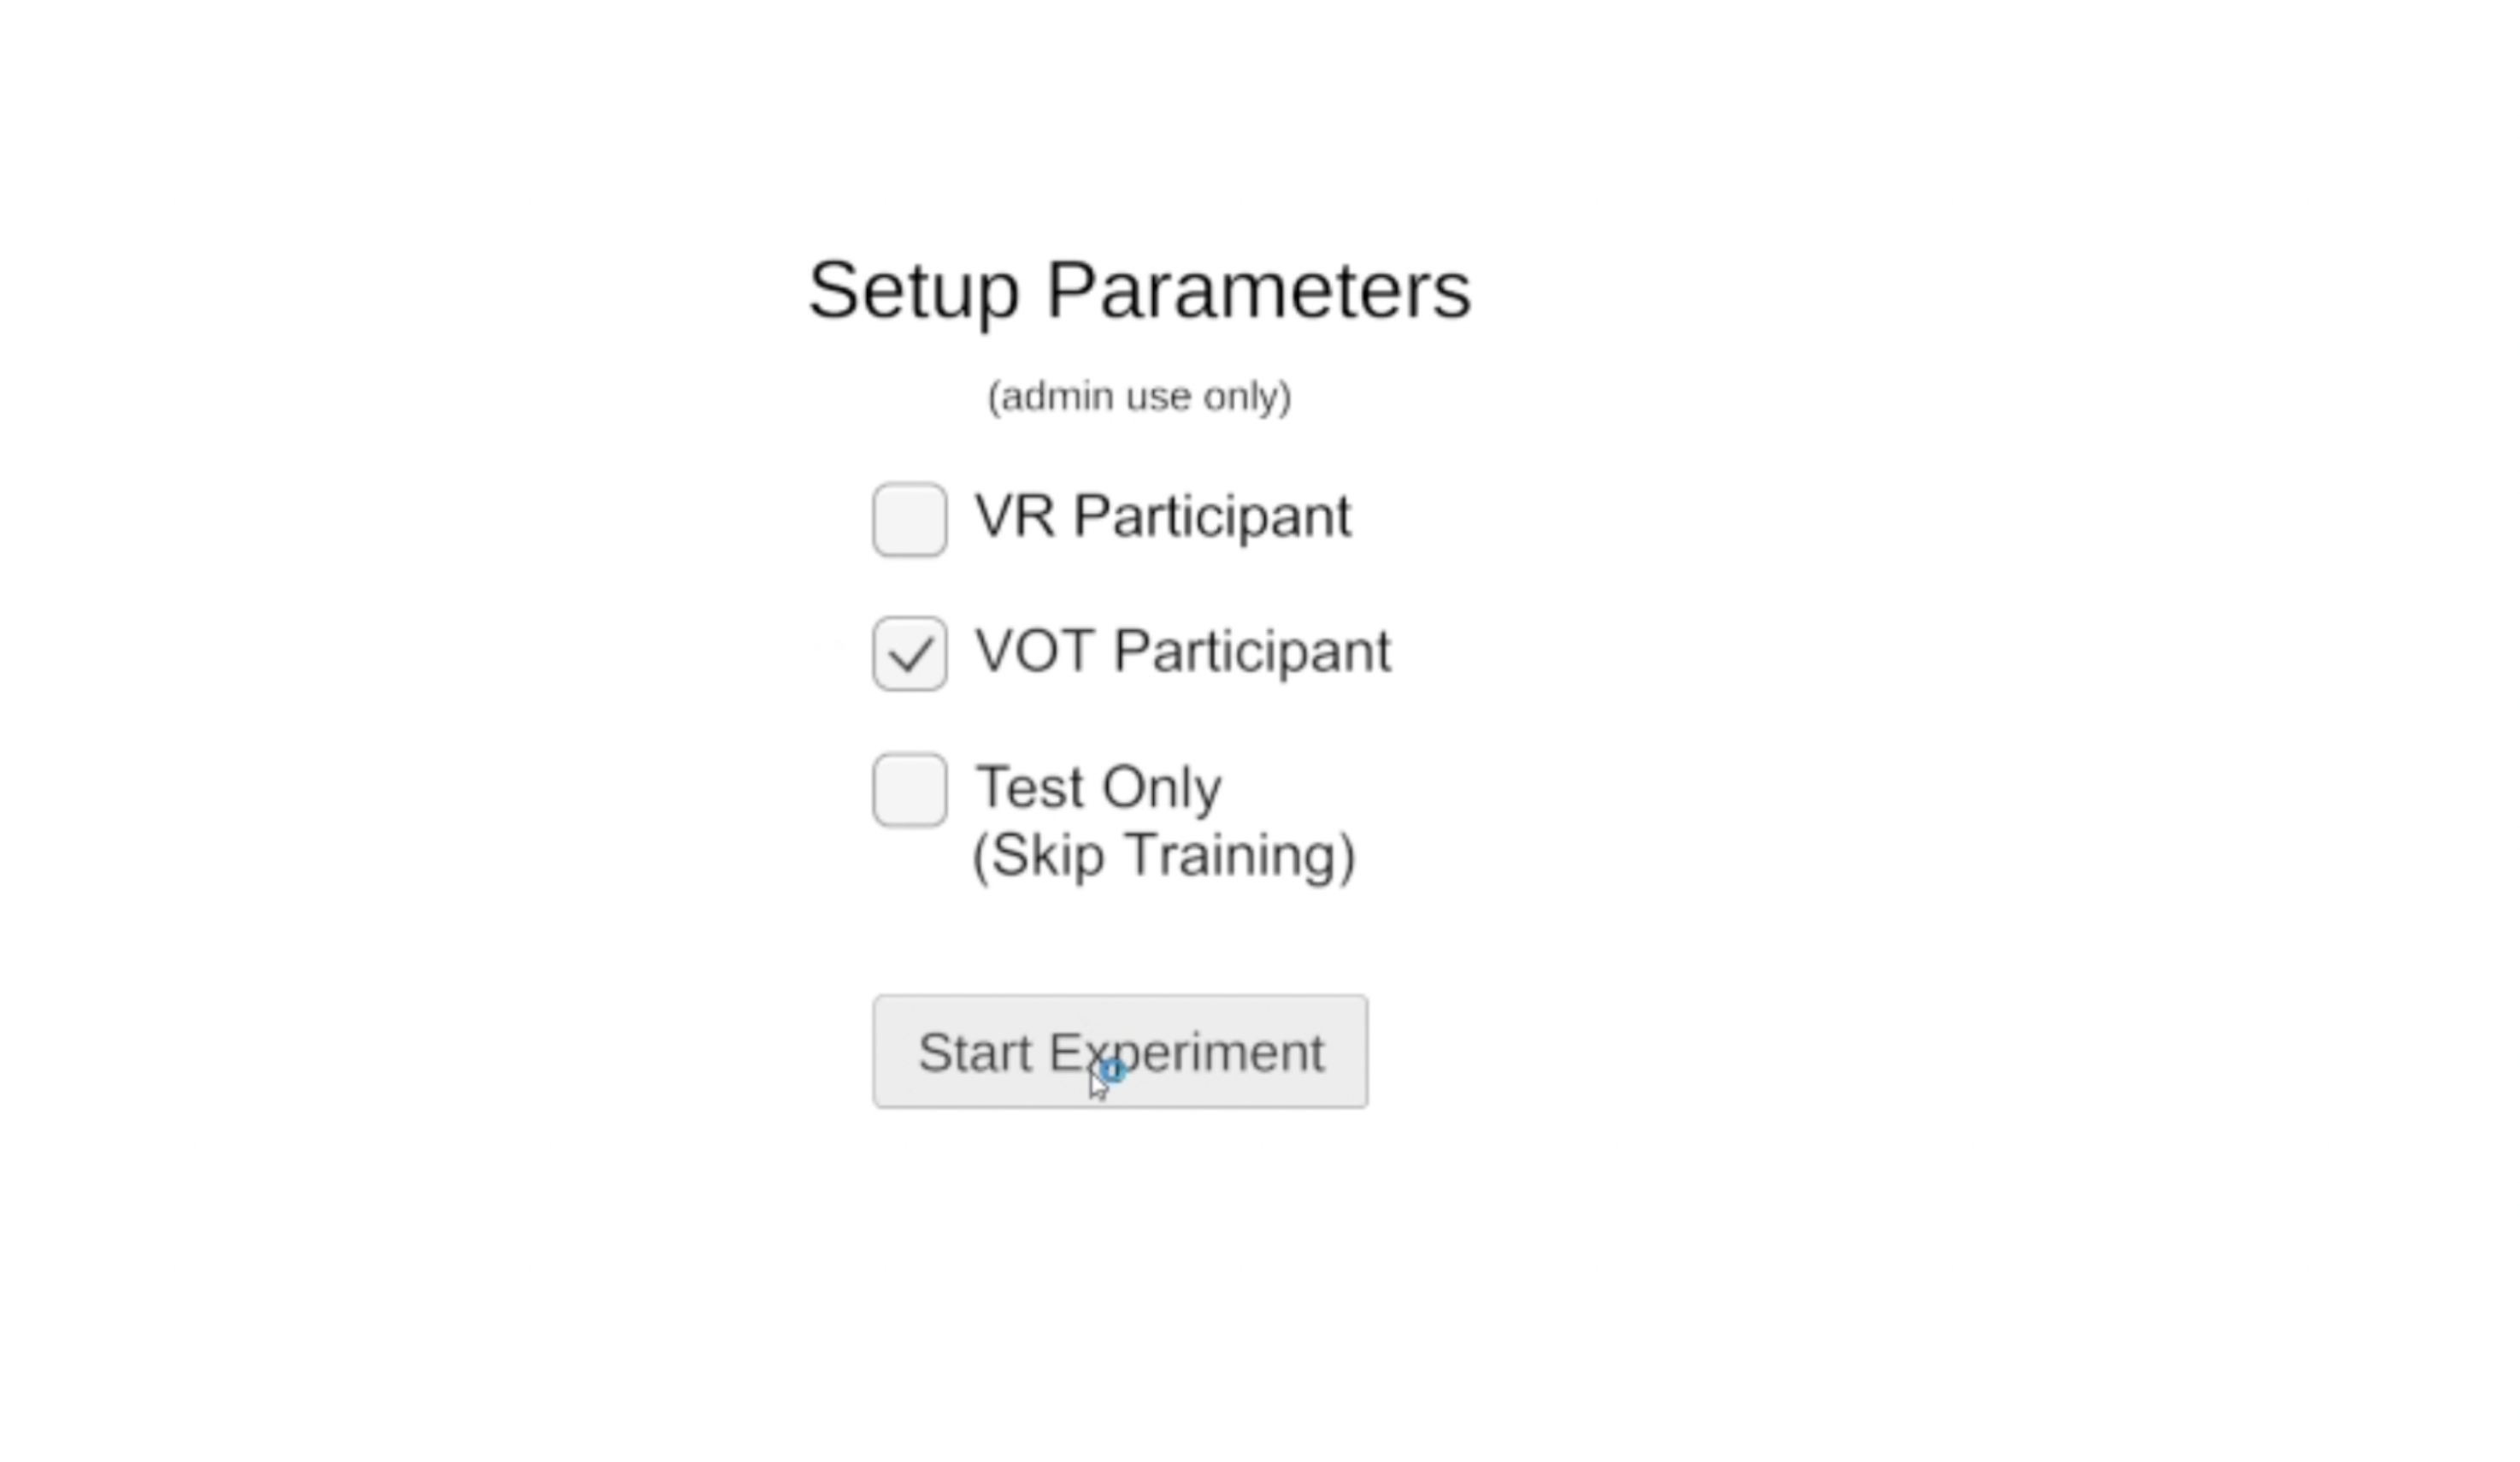
\includegraphics[width=\textwidth]{Photos/SB1.jpg}}
        \caption{Admin Setup}
        \label{fig:subim1}
    \end{subfigure}
    \hfill
    \begin{subfigure}[b]{0.3\textwidth}
        \fbox{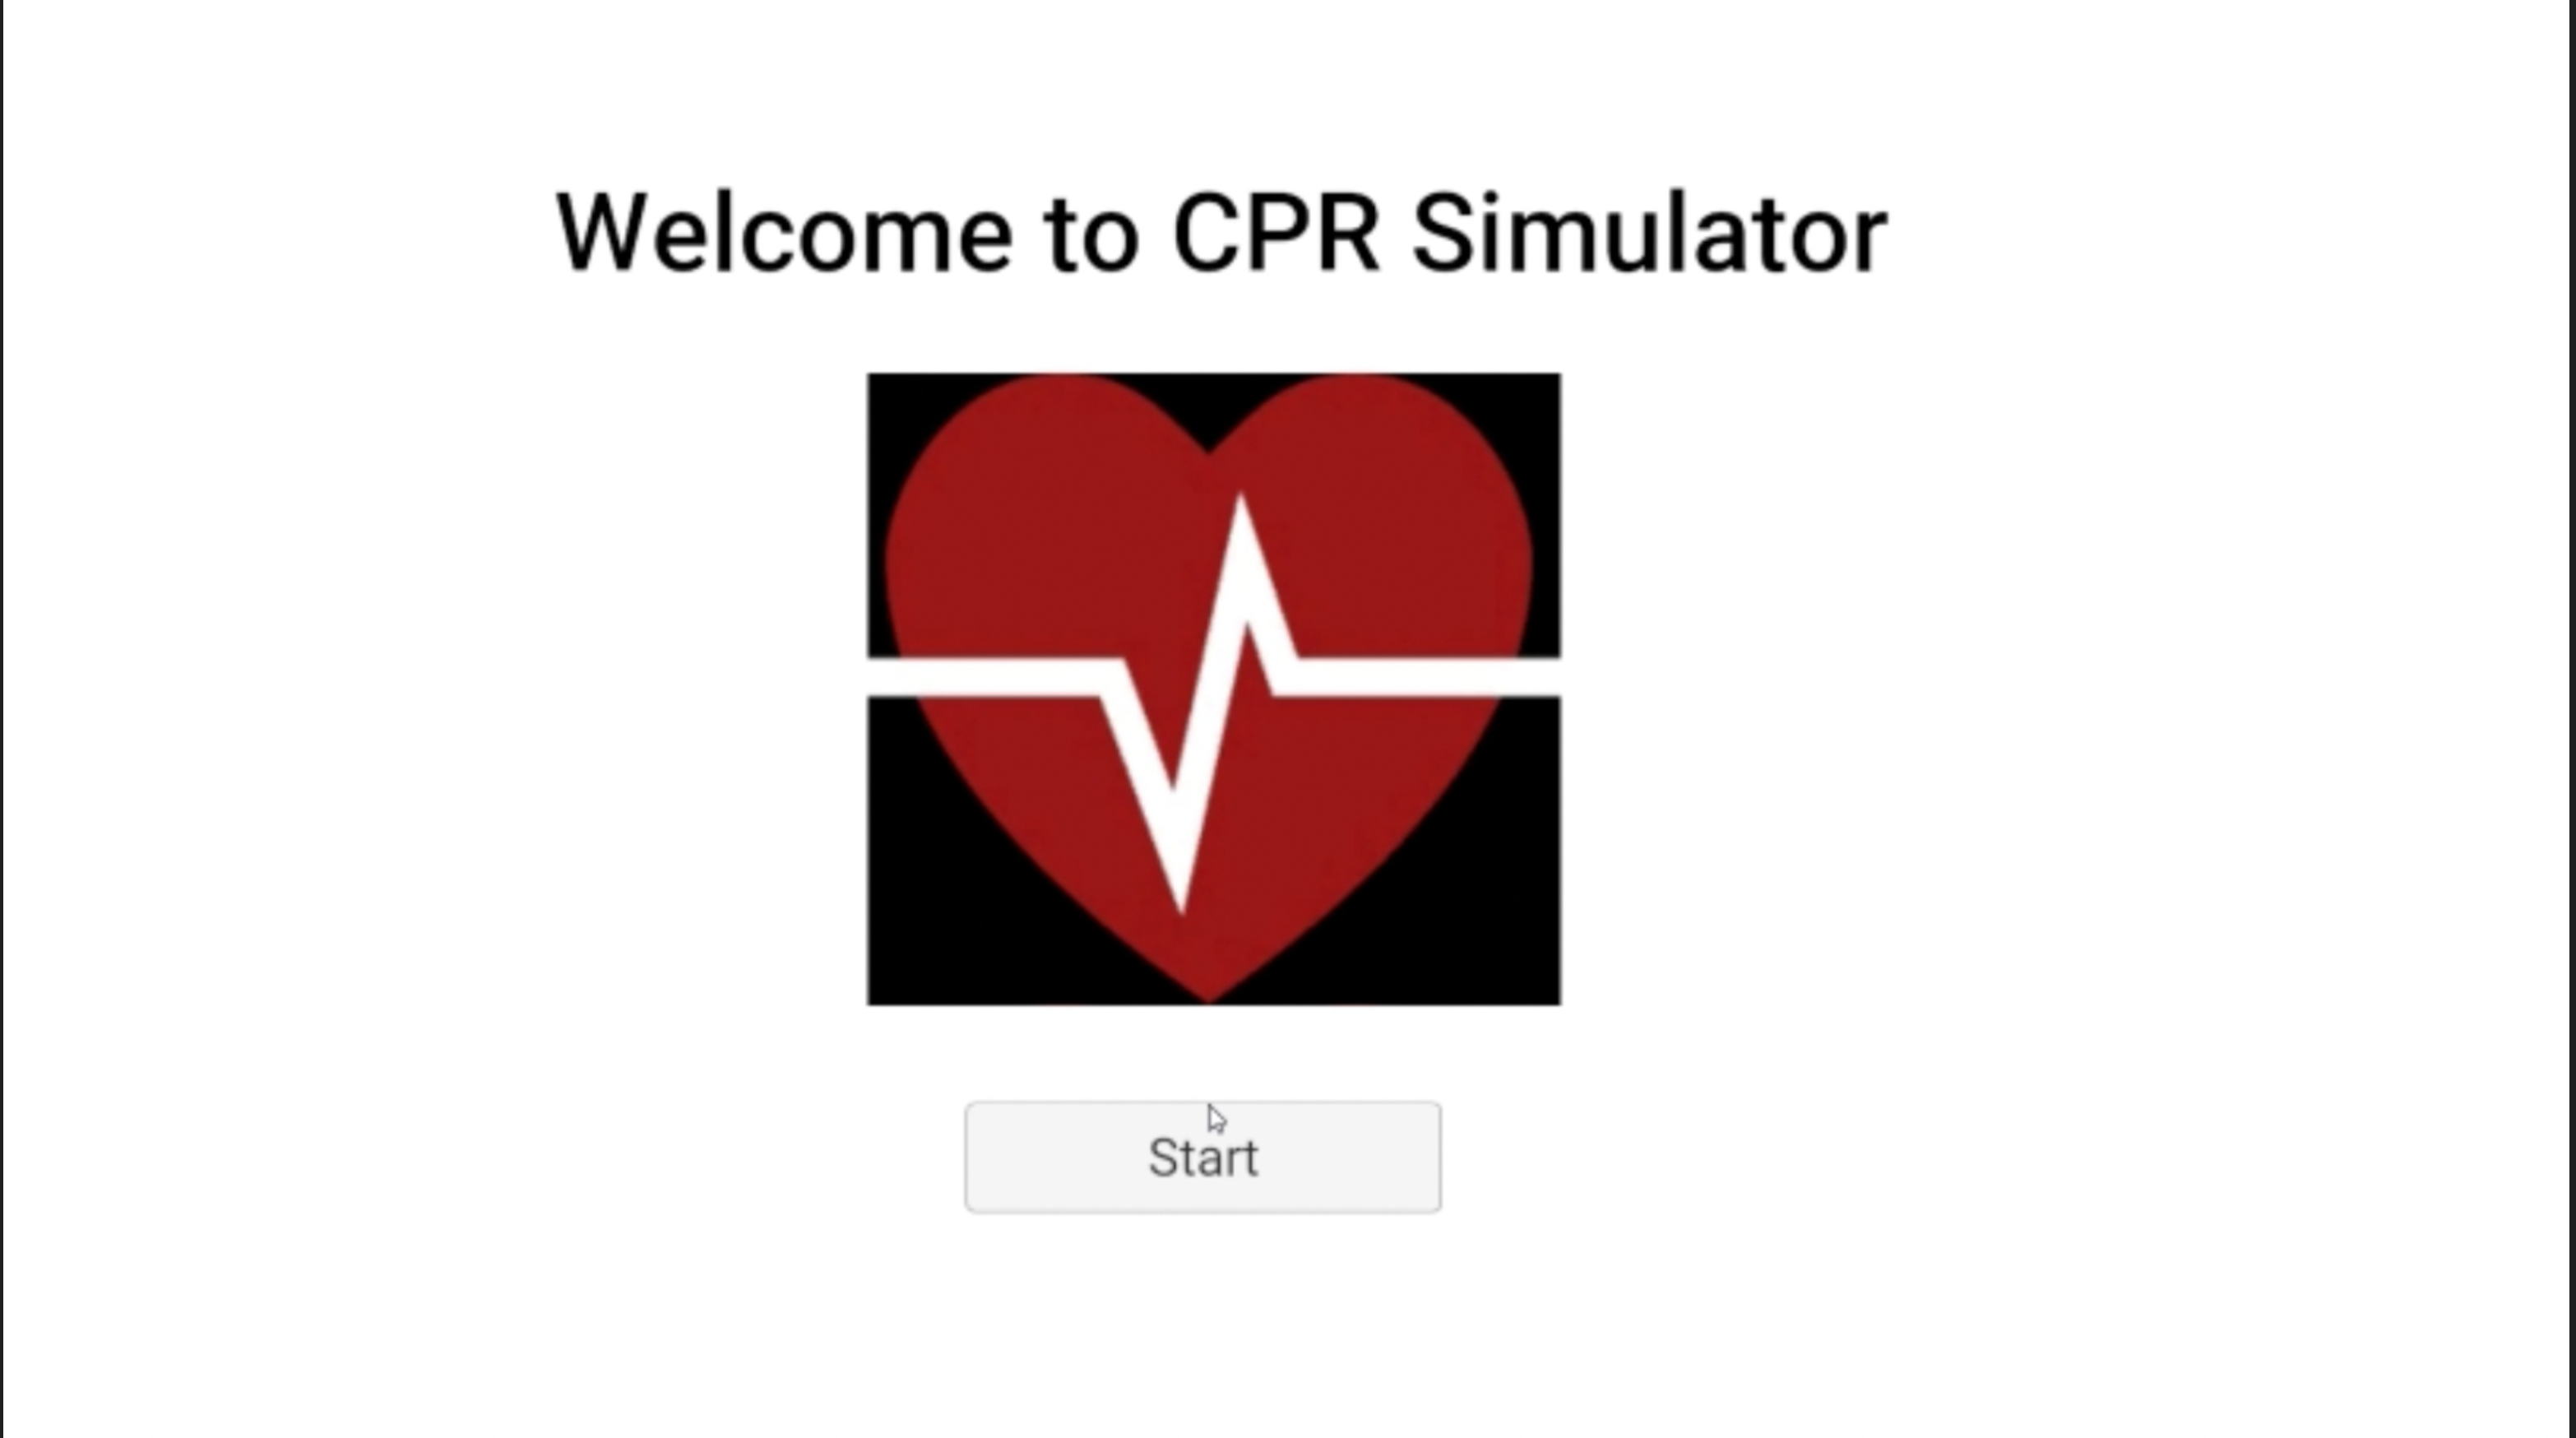
\includegraphics[width=\textwidth]{Photos/SB2.jpg}}
        \caption{Welcome}
        \label{fig:subim2}
    \end{subfigure}
    \hfill
    \begin{subfigure}[b]{0.3\textwidth}
        \fbox{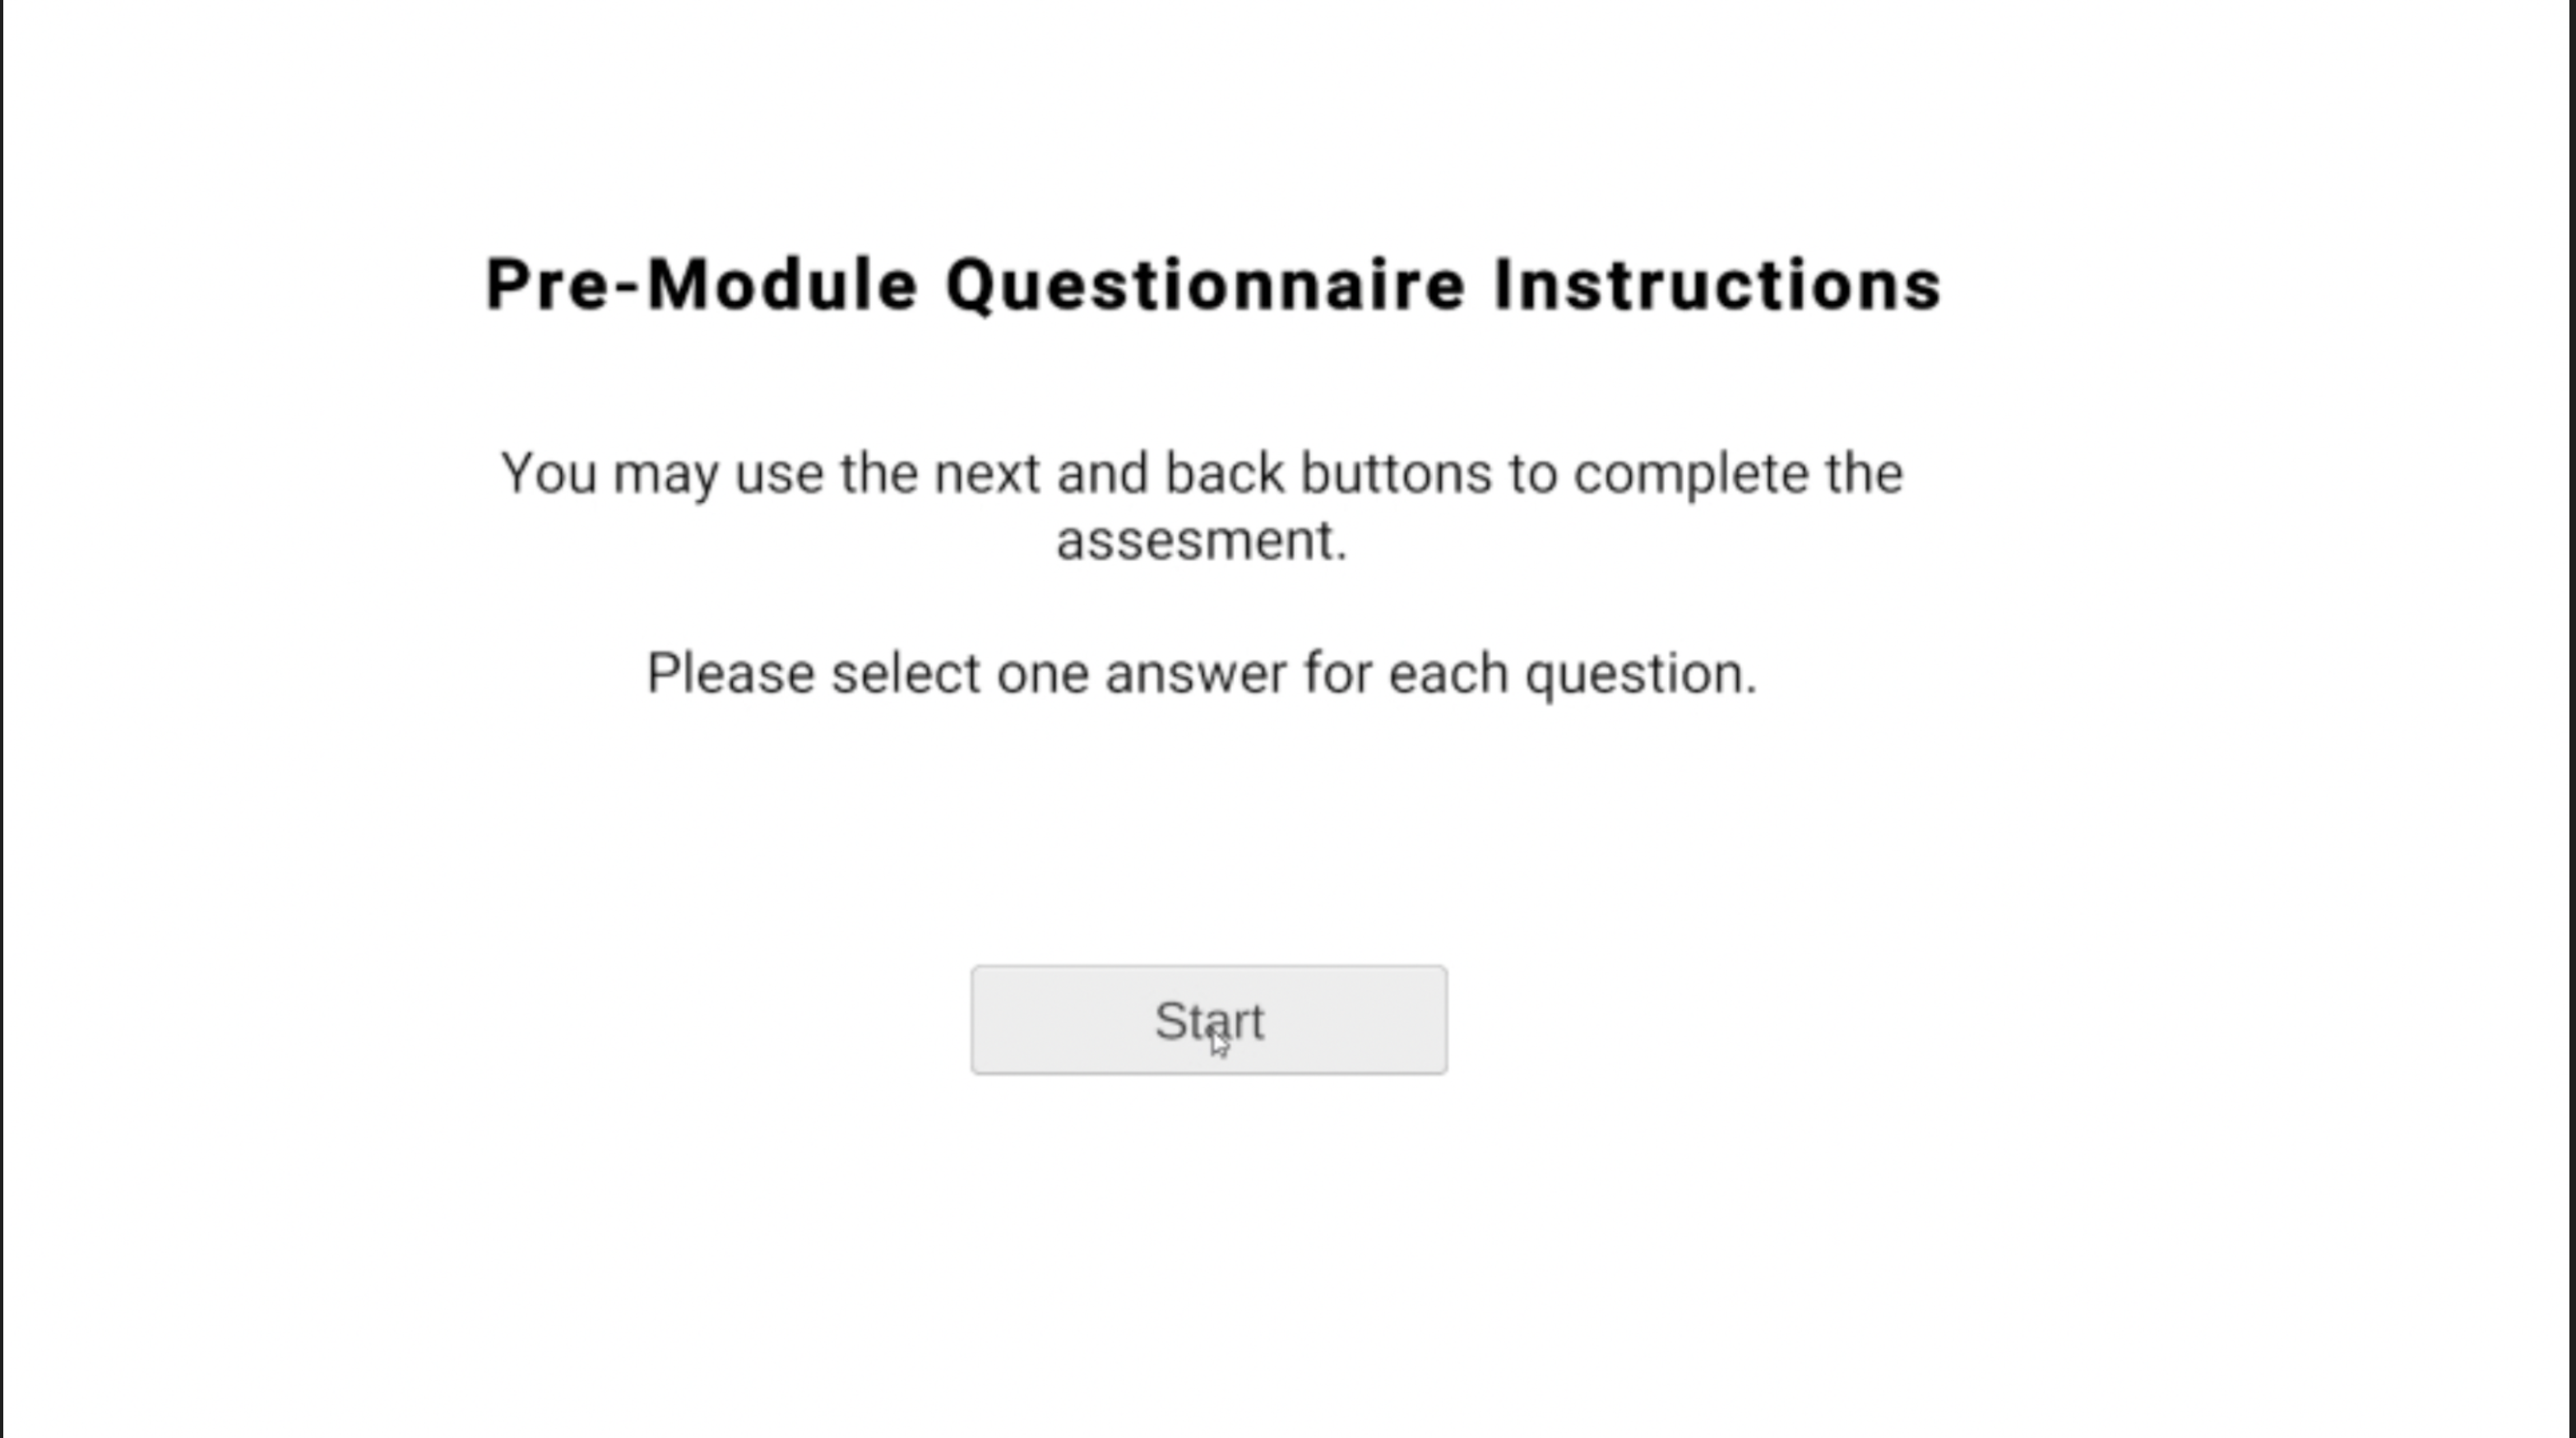
\includegraphics[width=\textwidth]{Photos/SB3.jpg}}
        \caption{Clear Instructions}
        \label{fig:subim3}
    \end{subfigure}
    \begin{subfigure}[b]{0.3\textwidth}
        \centering
        \fbox{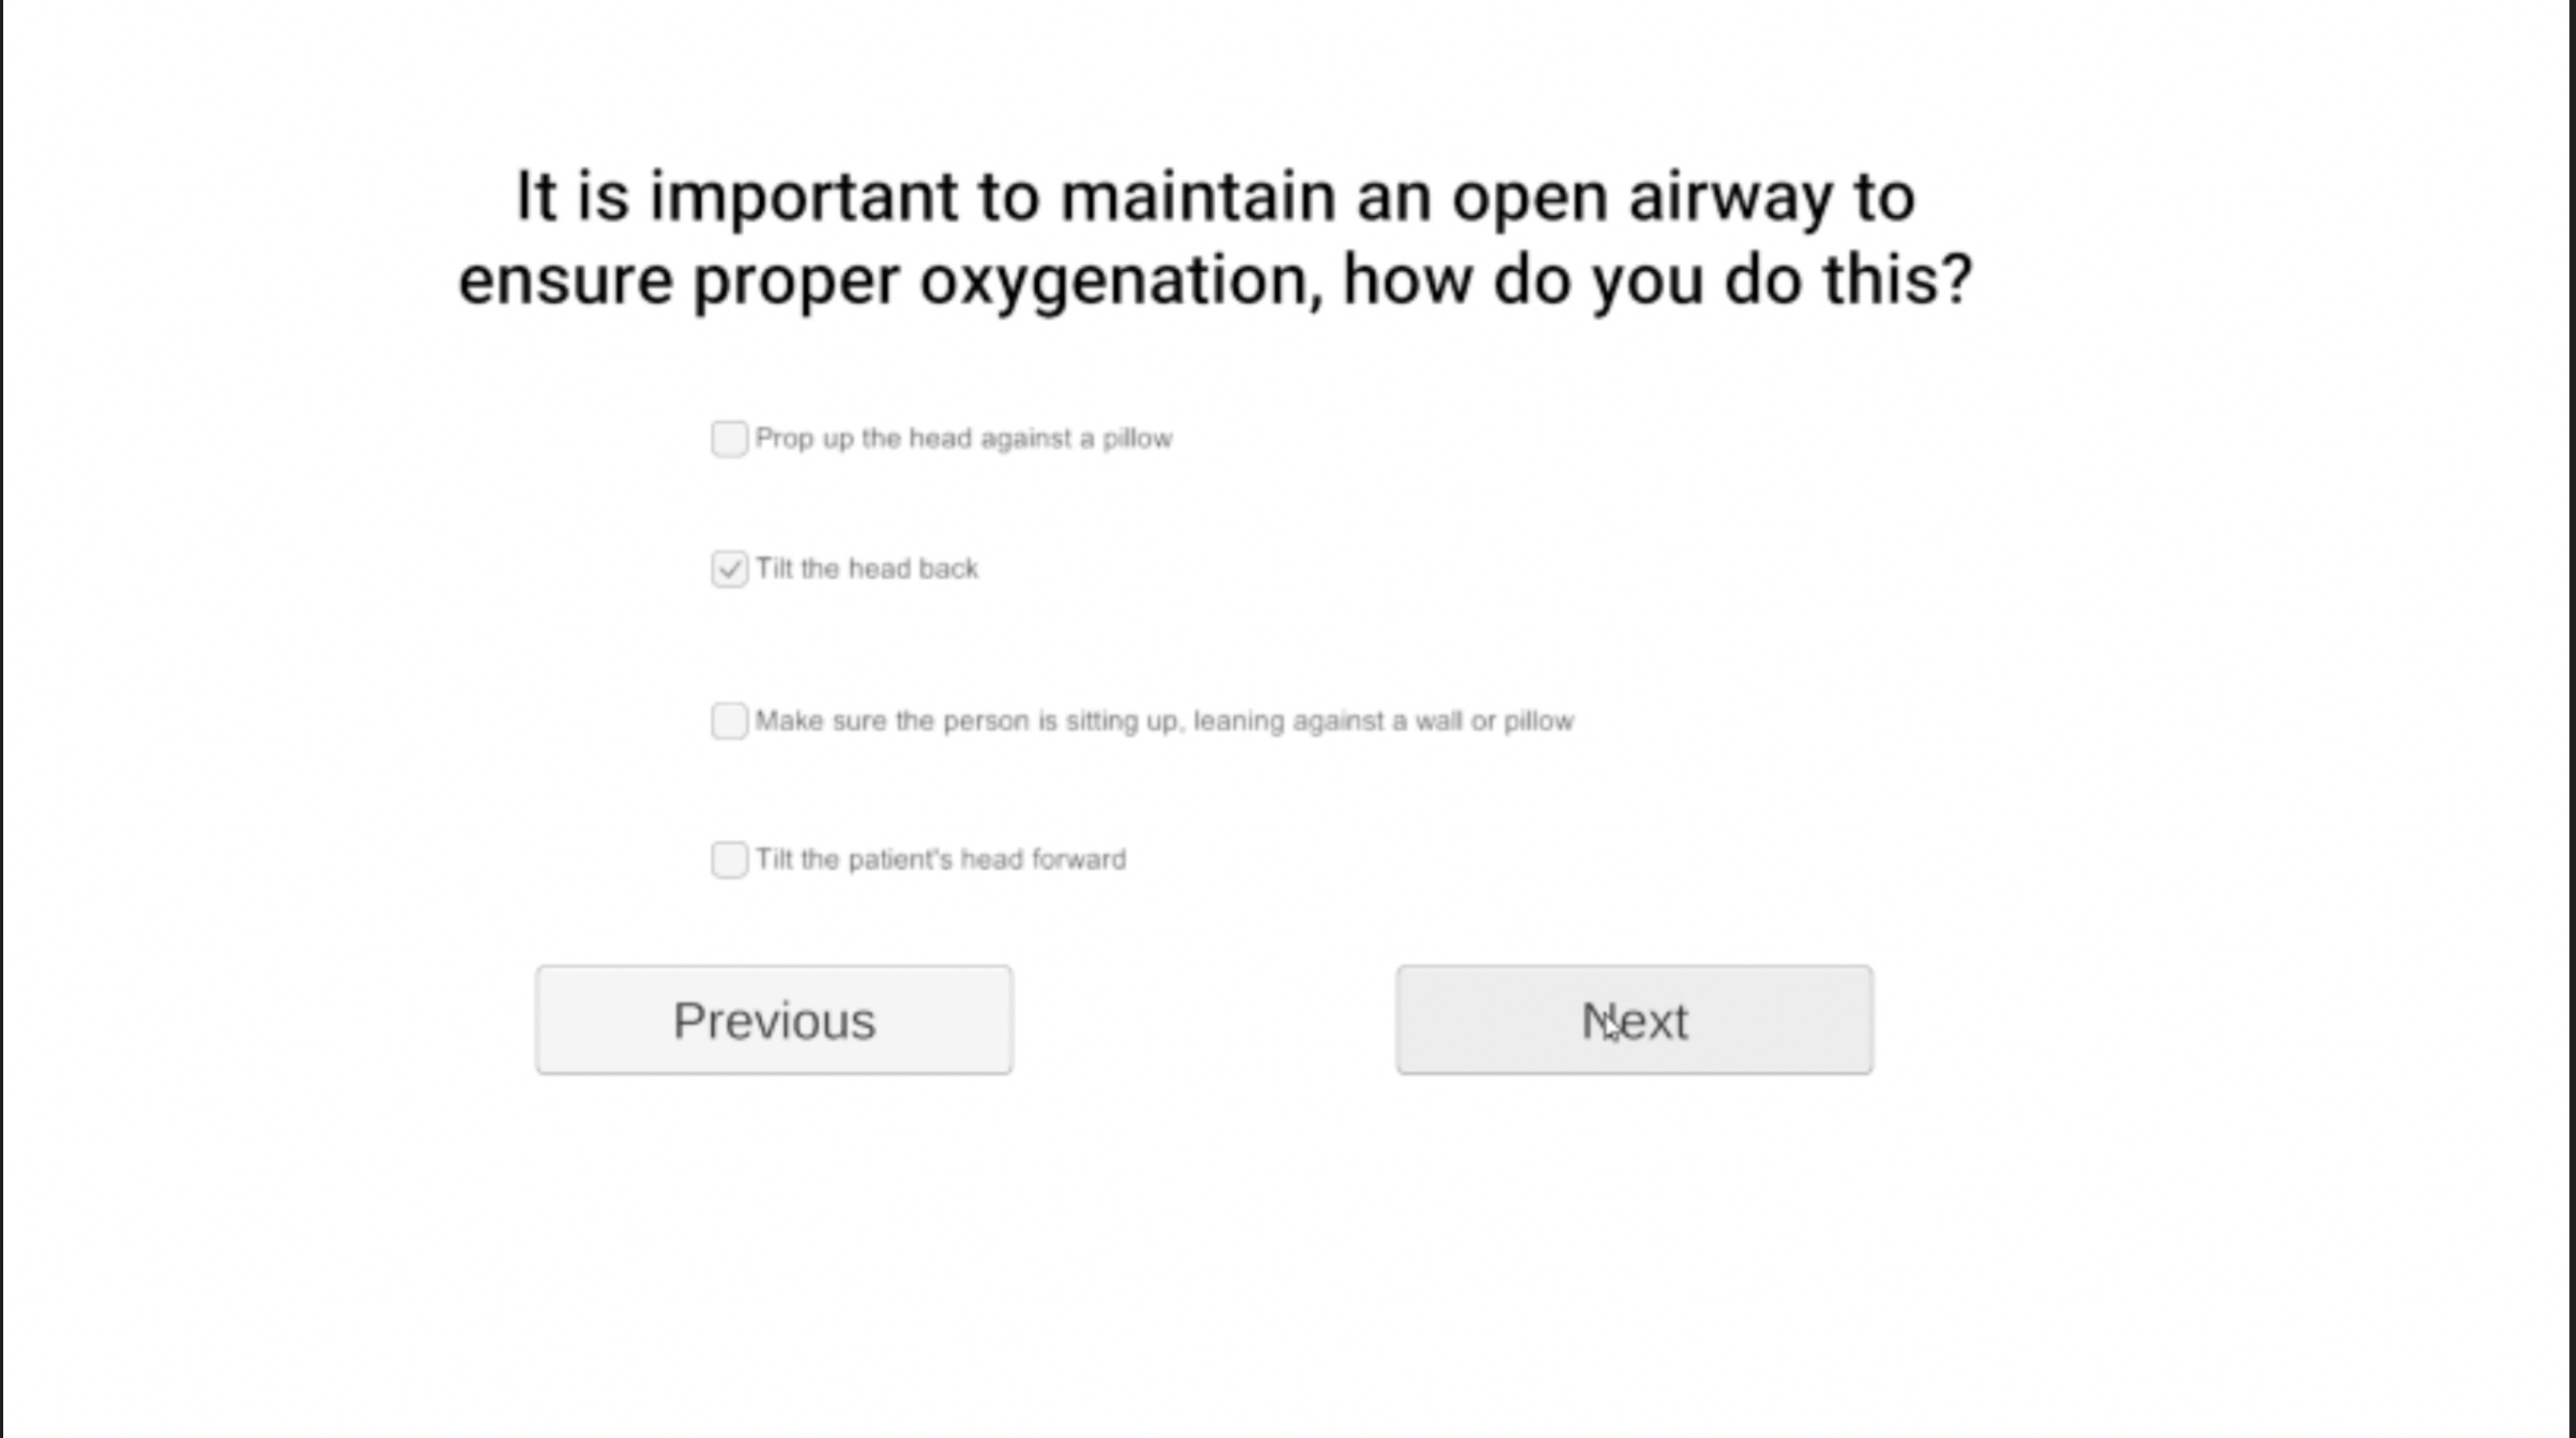
\includegraphics[width=\textwidth]{Photos/SB4.jpg}}
        \caption{Questionnaire Example}
        \label{fig:subim4}
    \end{subfigure}
    \hfill
    \begin{subfigure}[b]{0.3\textwidth}
        \fbox{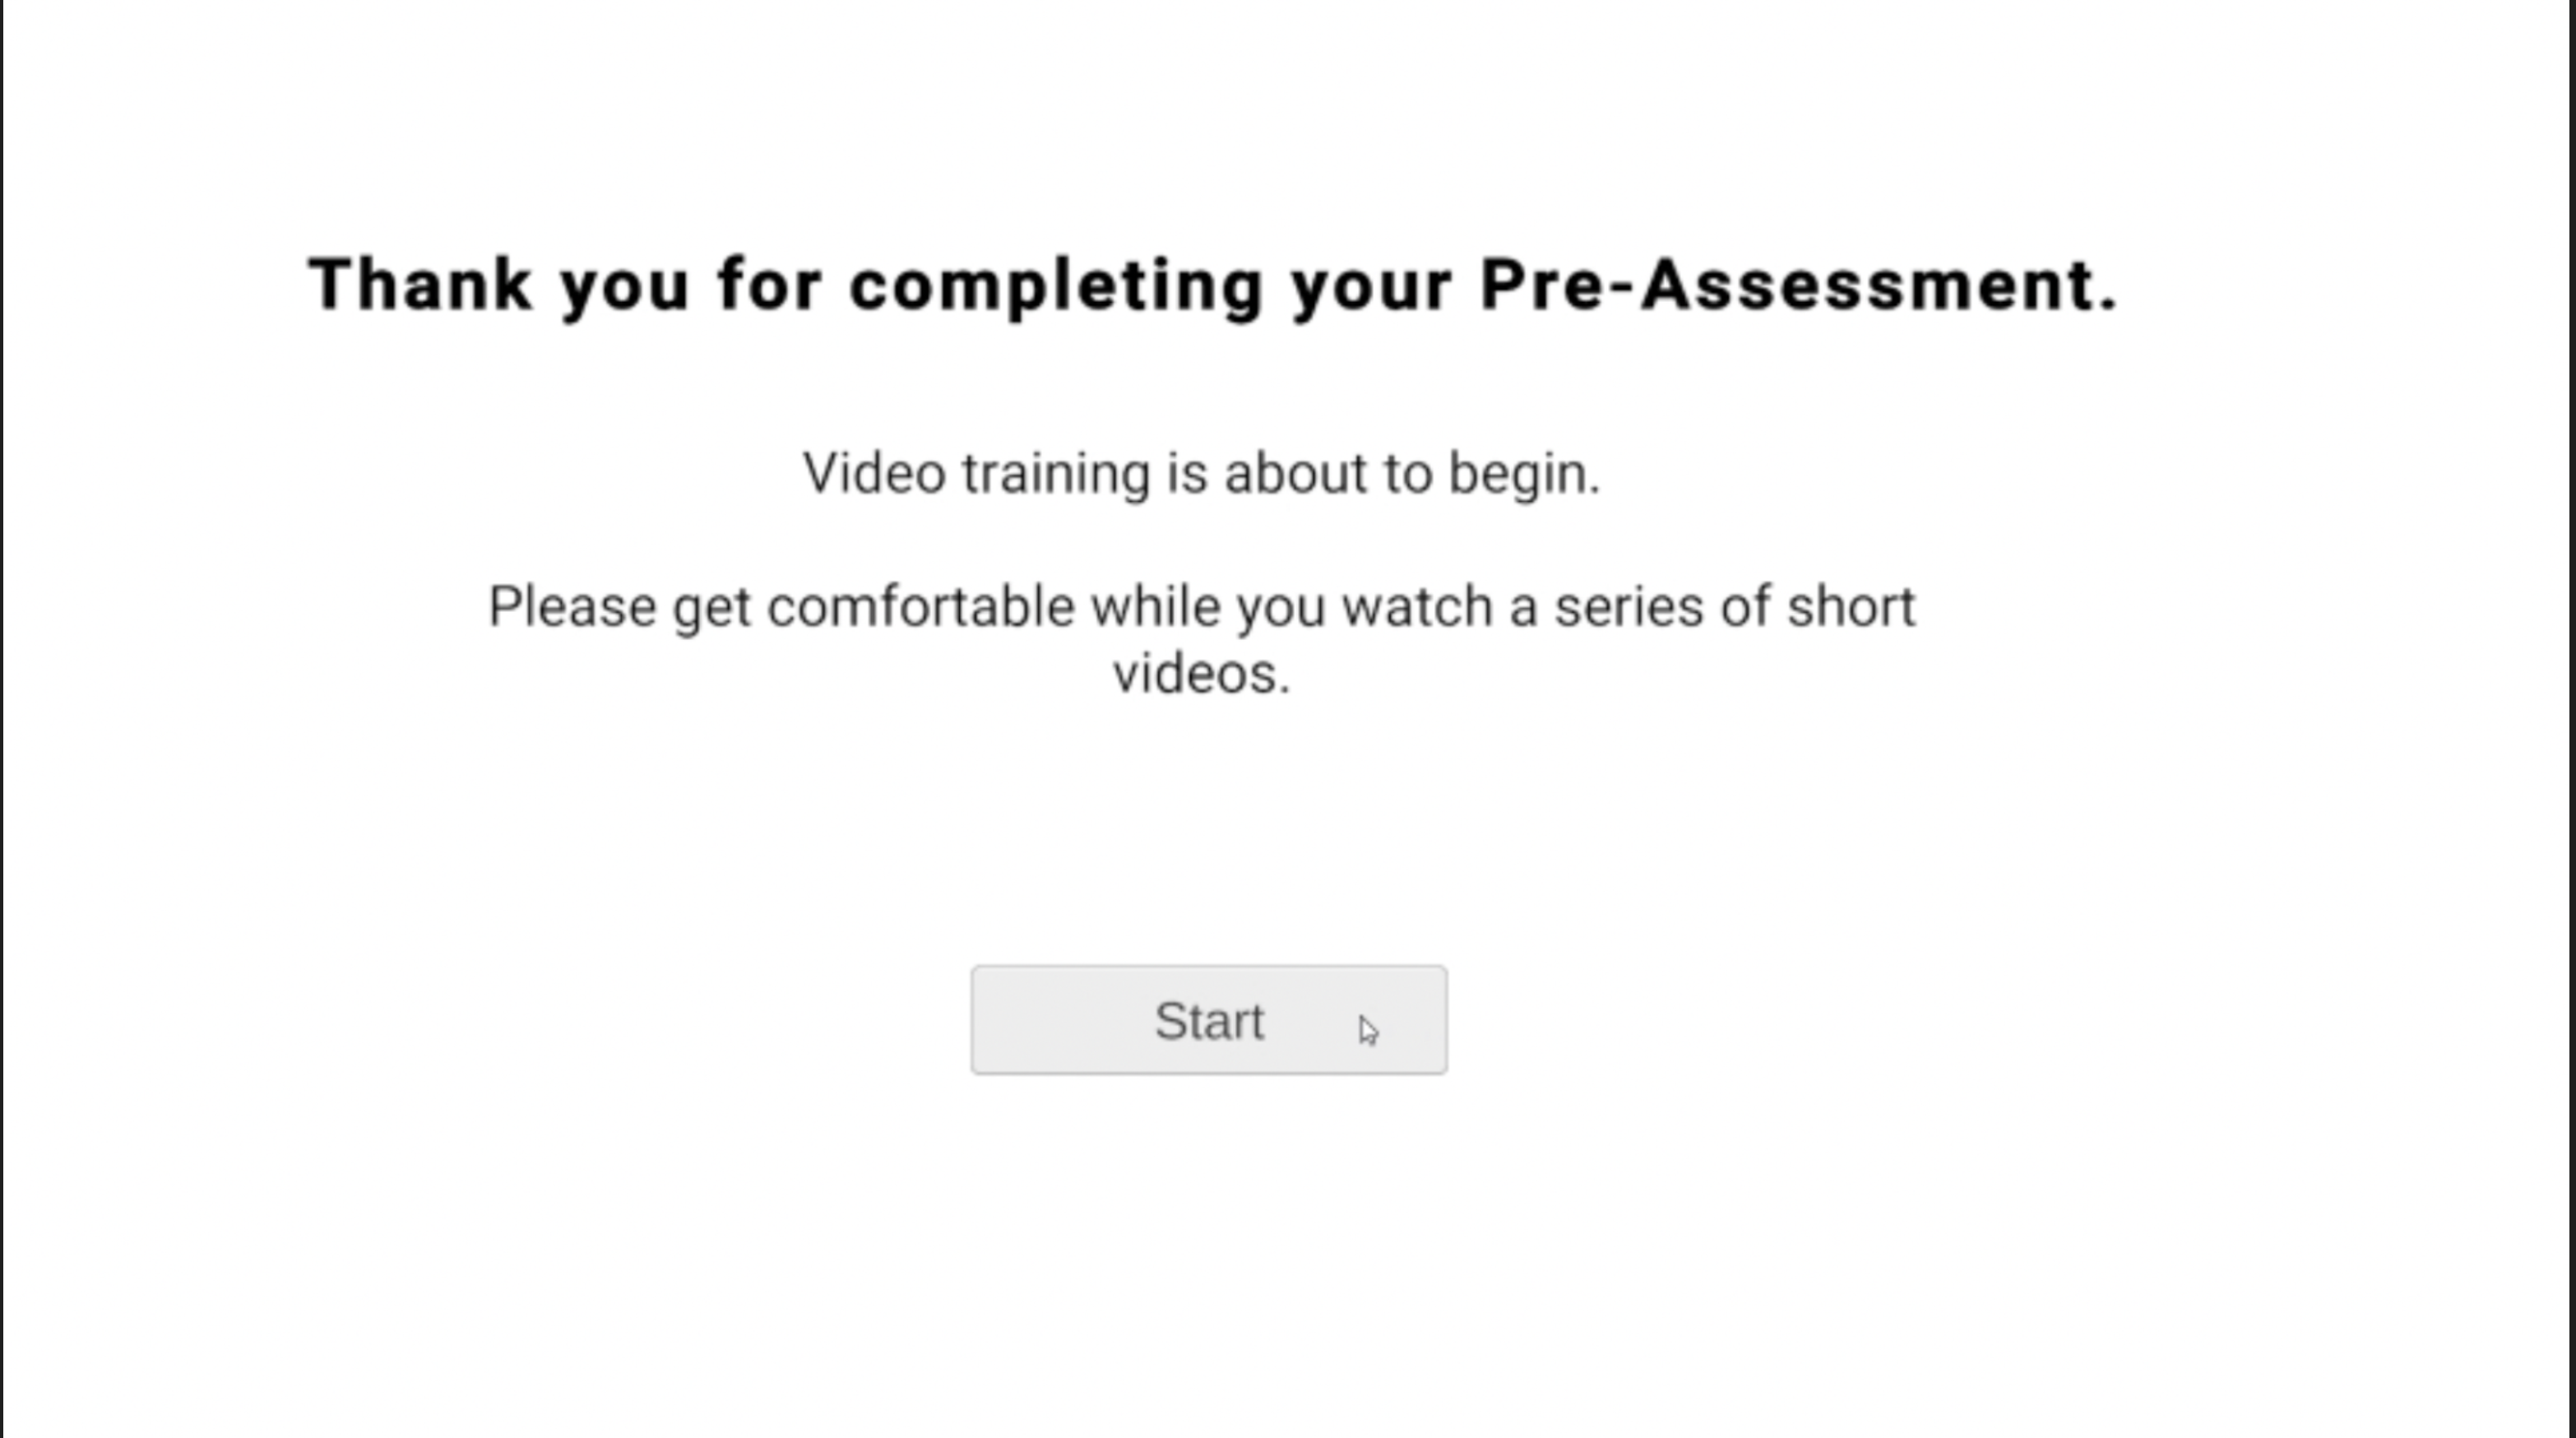
\includegraphics[width=\textwidth]{Photos/SB5.jpg}}
        \caption{Assessment Completion}
        \label{fig:subim5}
    \end{subfigure}
    \hfill
    \begin{subfigure}[b]{0.3\textwidth}
        \fbox{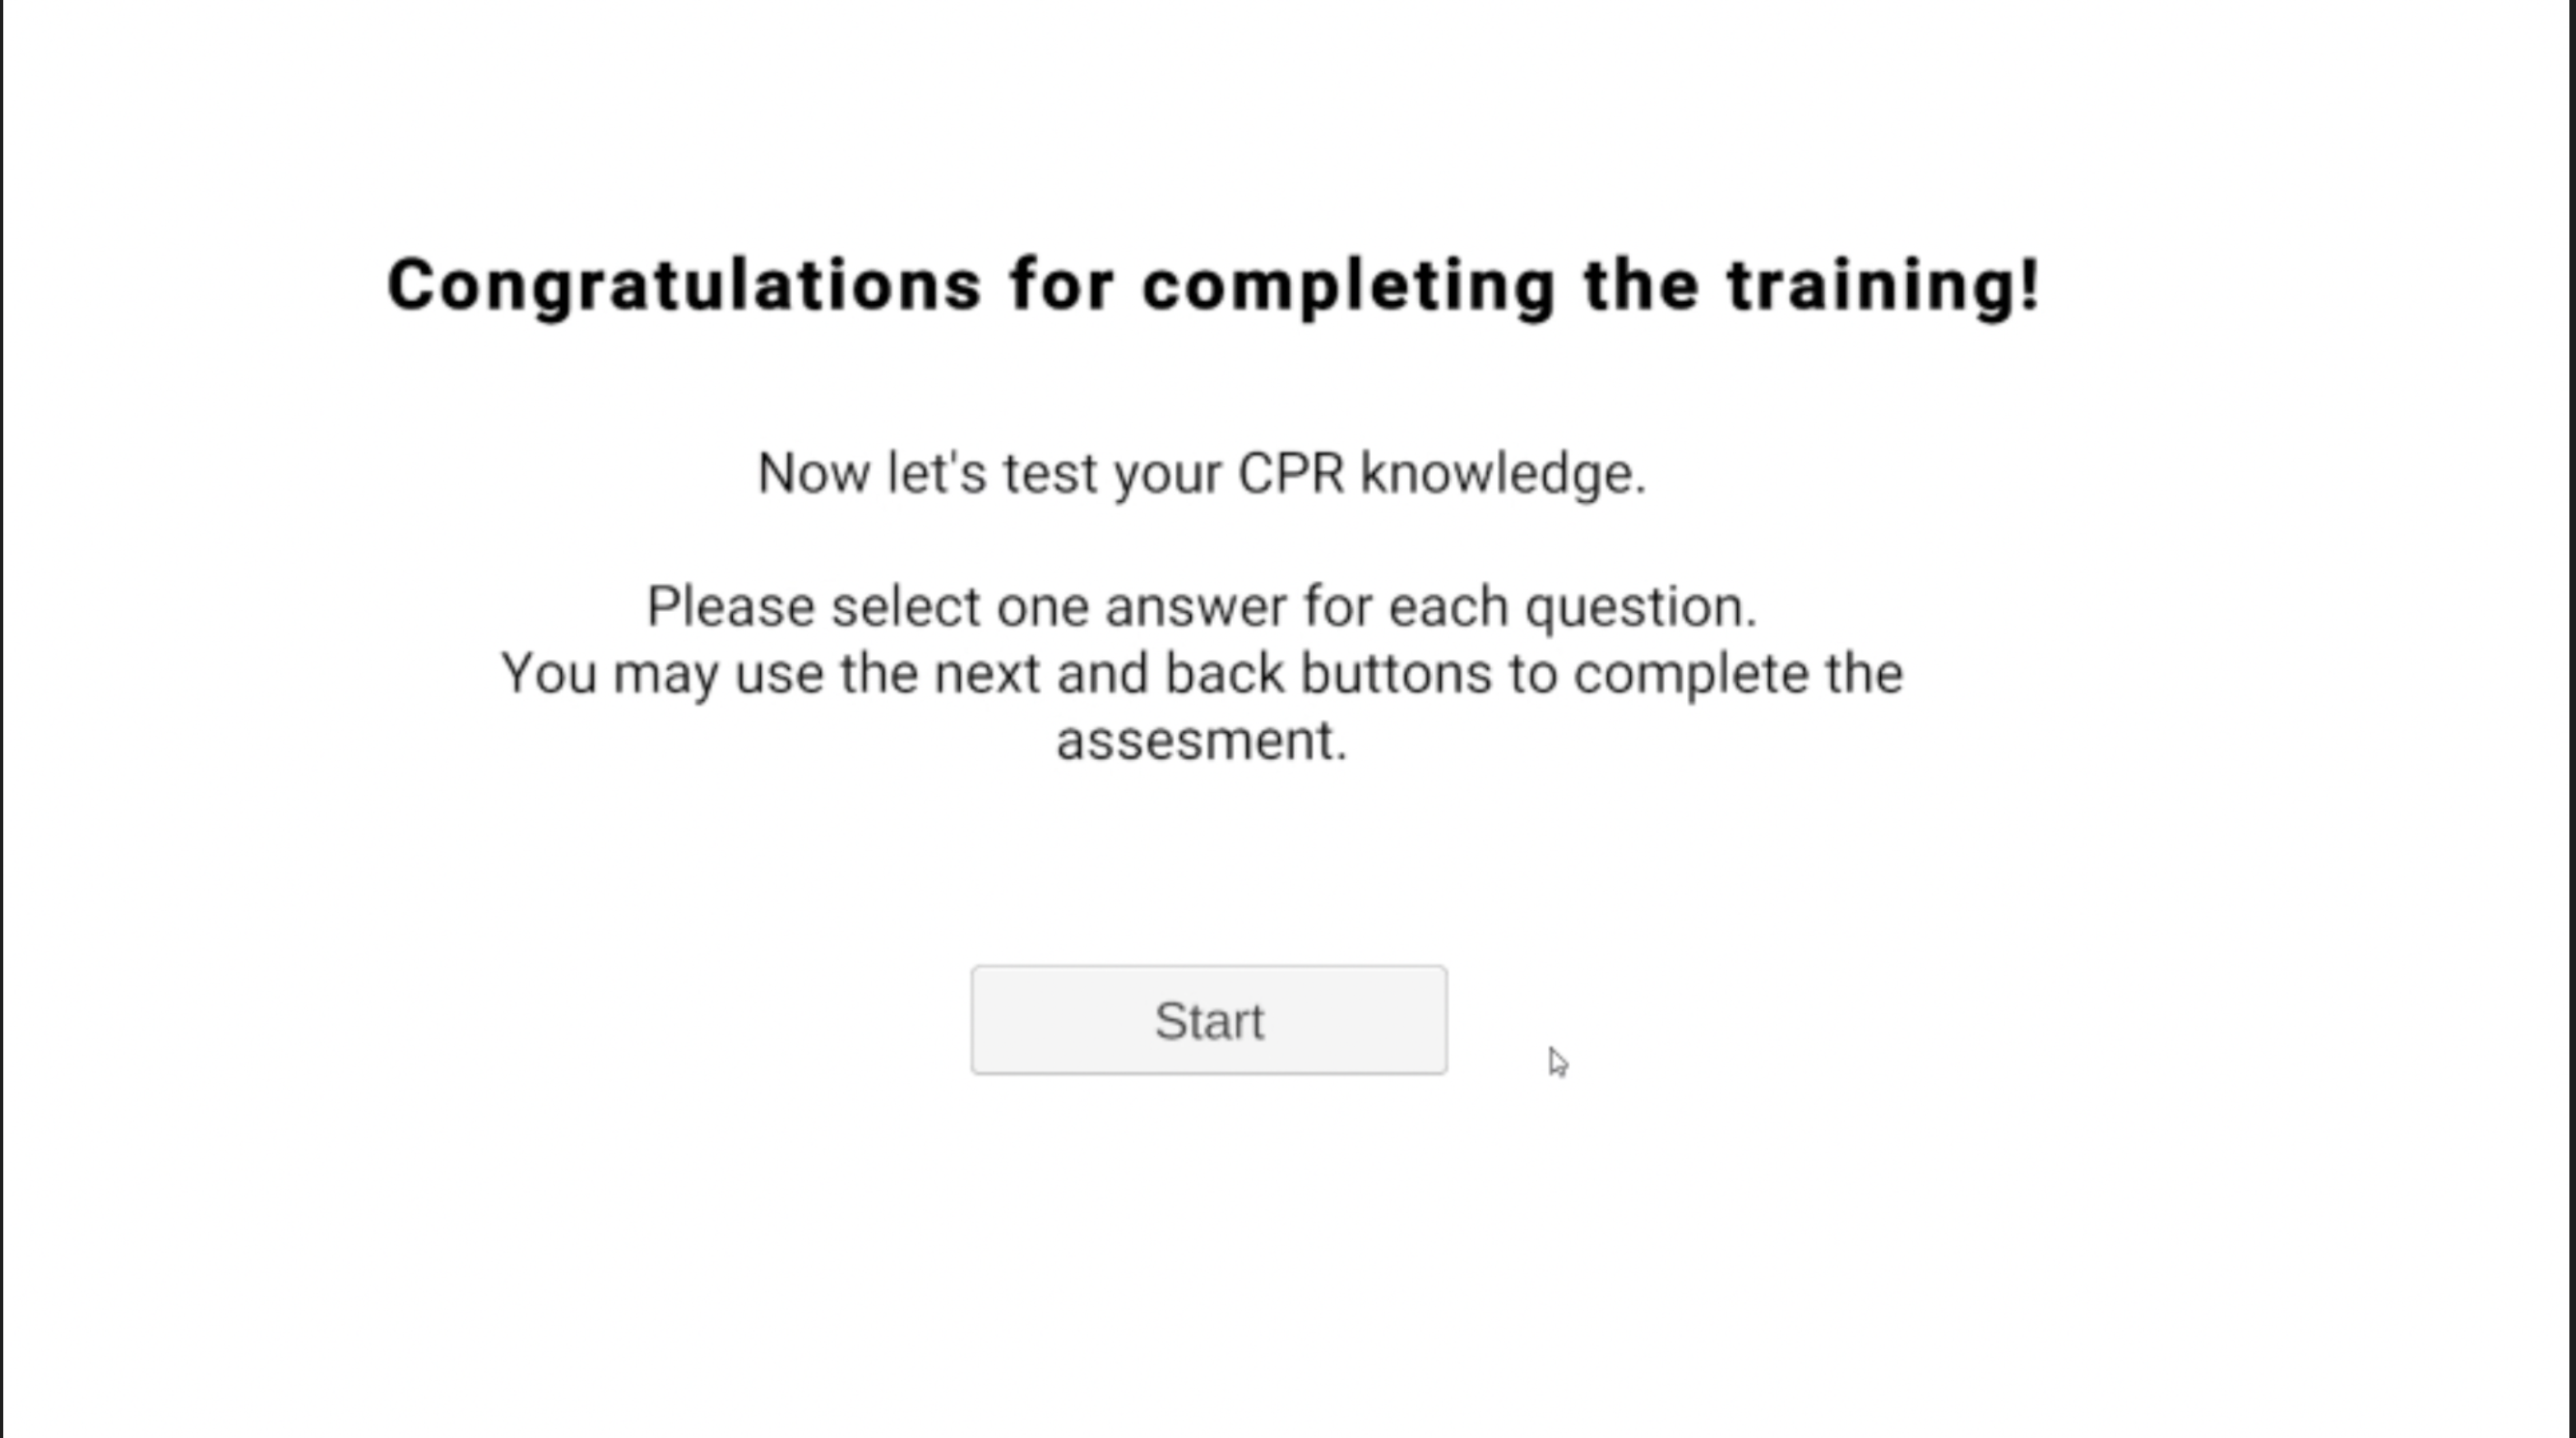
\includegraphics[width=\textwidth]{Photos/SB6.jpg}}
        \caption{Training Completion}
        \label{fig:subim6}
    \end{subfigure}
        \caption{2D screen-to-screen transition and text examples}
        \label{fig: second three screens}
\end{figure}

The Unity project was developed to accommodate both the control group as well as the experimental group. That is, the application randomly assigns the participant to one of the two groups and then guides the participant through one of two tutorials: the video observation path or the VR path, depending on which group they were assigned to. The control group was instructed to watch a four-minute video, while the experimental group was tasked with physically performing CPR step-by-step in a VR environment, which averaged between four and six minutes to complete. See Figure \ref{fig:overallVR} for the VR scene screenshots. After completing their assigned training method, each participant was administered the same test to assess comprehension. Given the brevity of the study, no rest period was facilitated mid-experiment.

 \begin{figure}[h]
    \centering
    \begin{subfigure}[b]{0.24\textwidth}
        \centering
        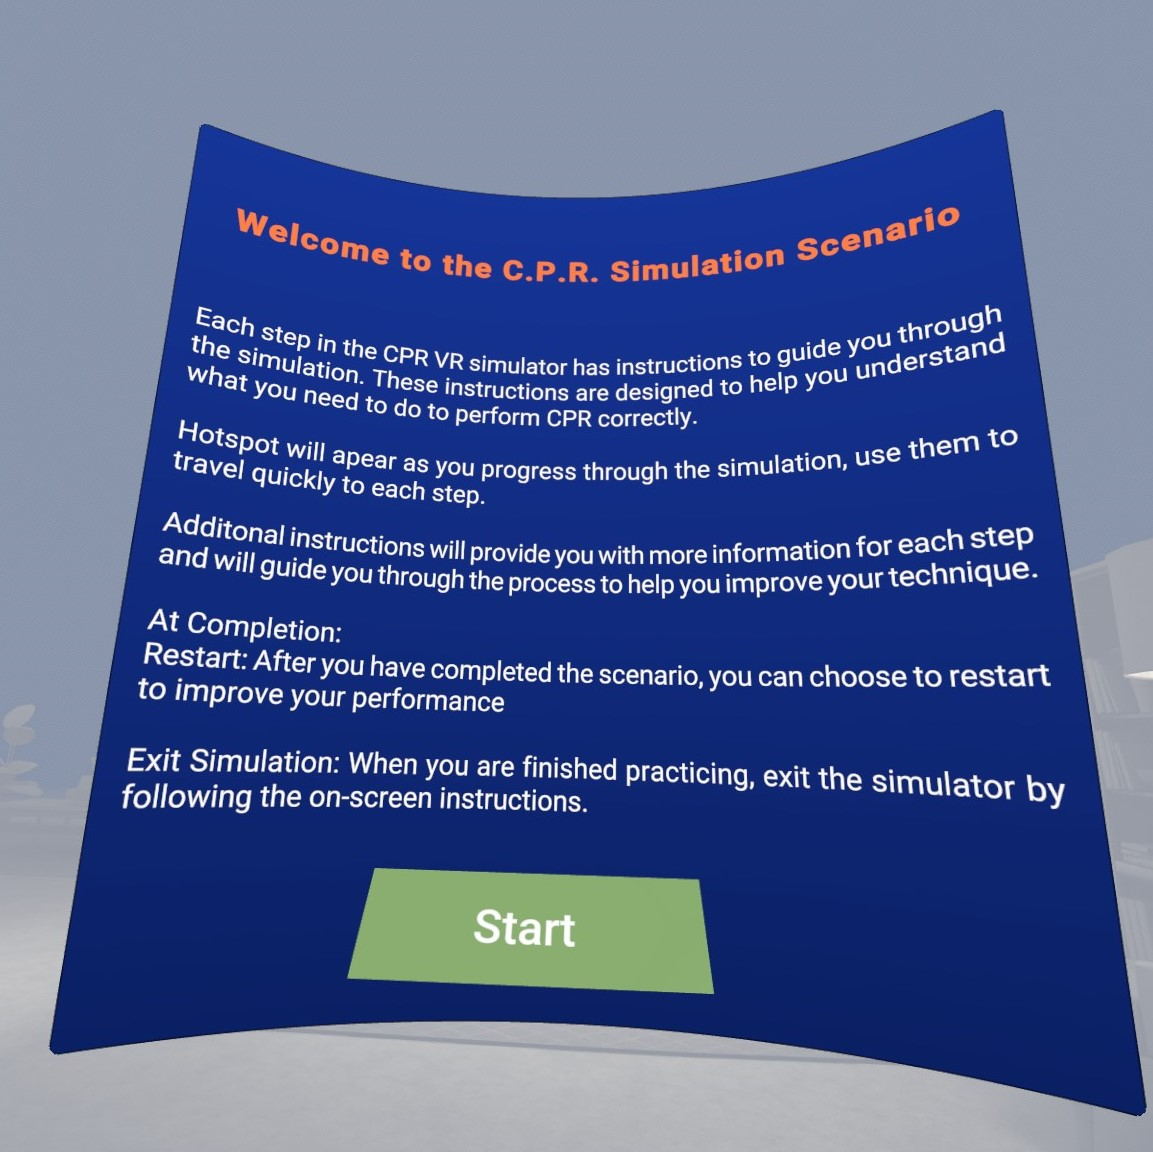
\includegraphics[width=\textwidth]{Photos/VR1.jpeg}
        \caption{Instructional Board}
        \label{fig:VR1}
    \end{subfigure}
    \hfill
    \begin{subfigure}[b]{0.24\textwidth}
        \centering
        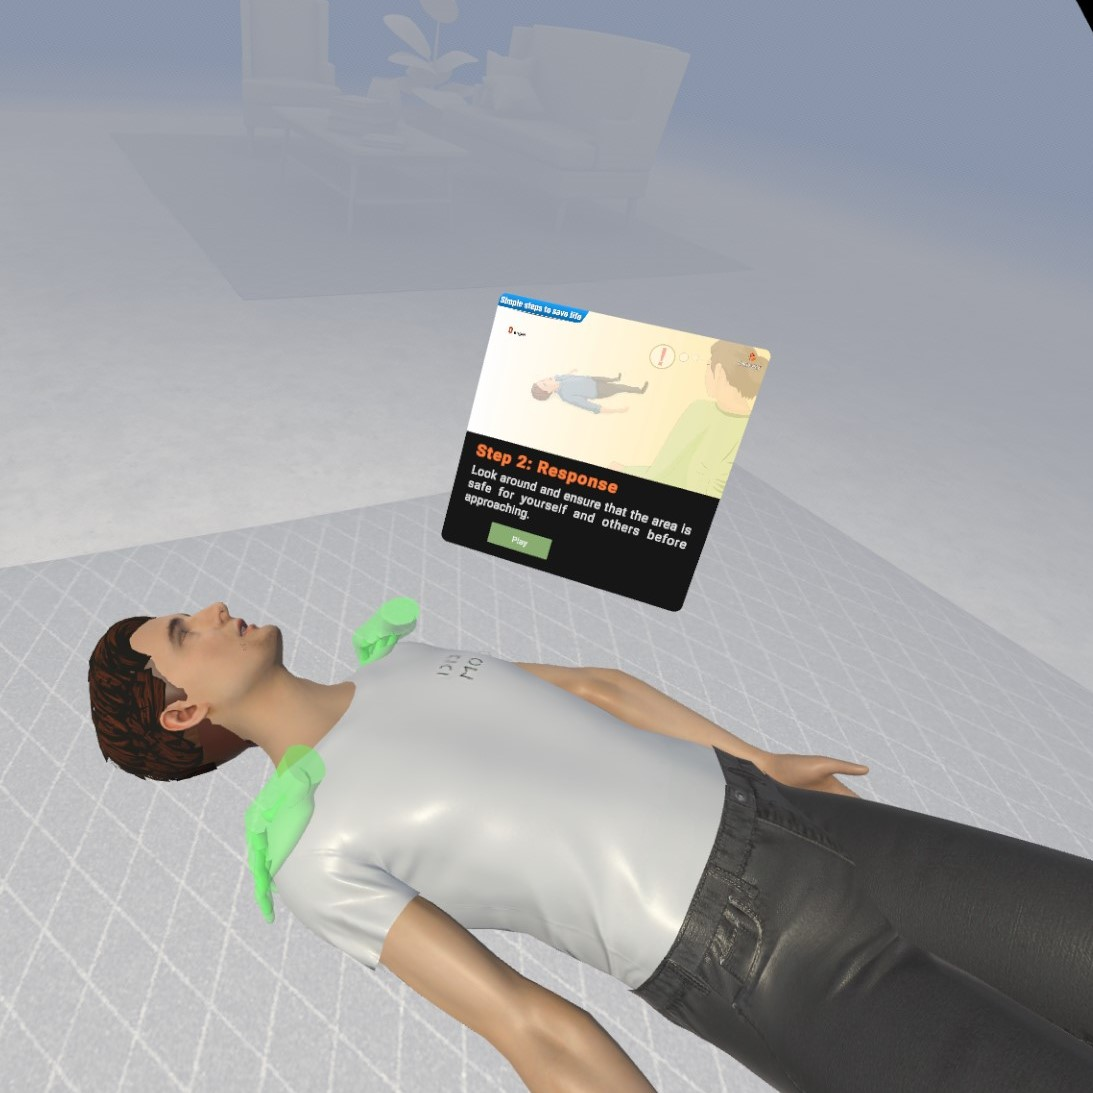
\includegraphics[width=\textwidth]{Photos/VR2.jpeg}
        \caption{Mock hand placement}
        \label{fig:VR2}
    \end{subfigure}
    \hfill
    \begin{subfigure}[b]{0.24\textwidth}
        \centering
        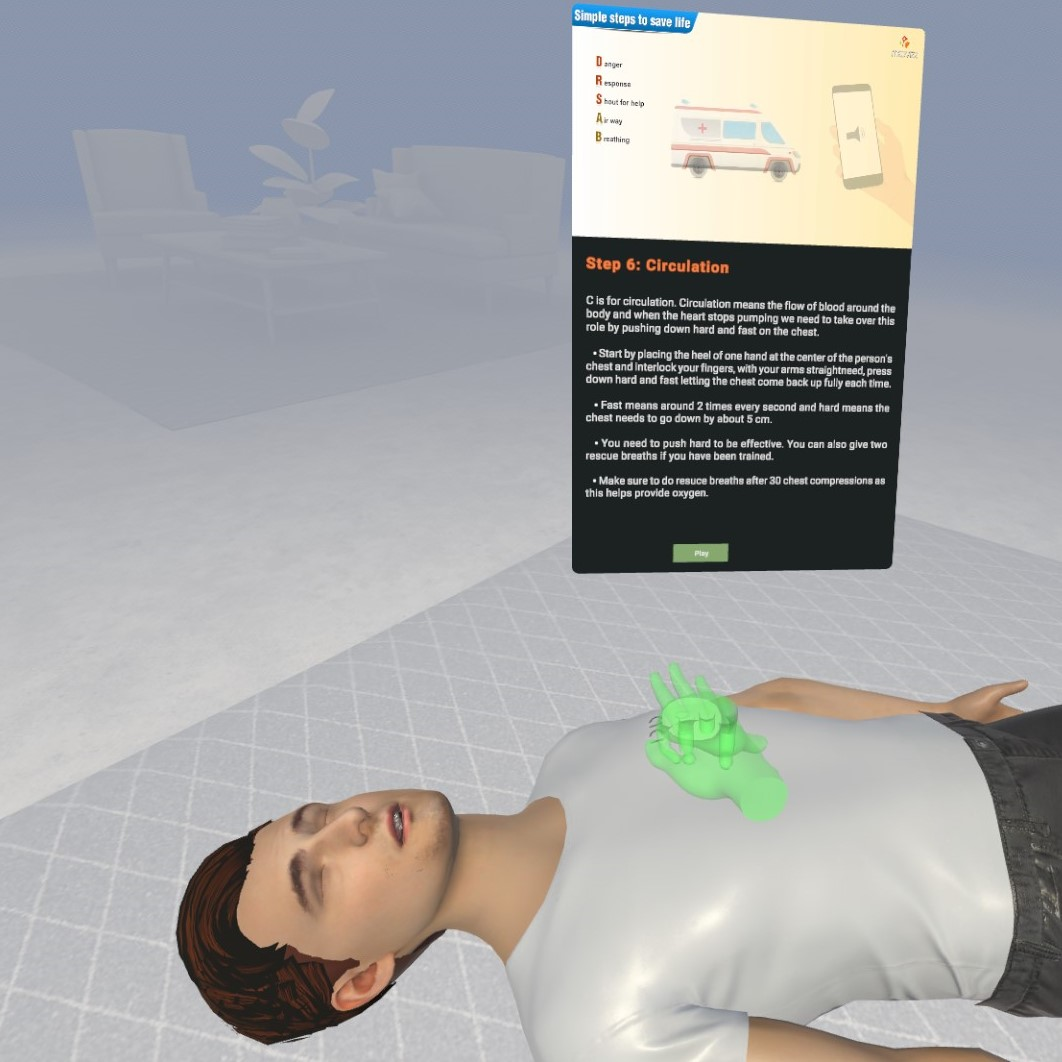
\includegraphics[width=\textwidth]{Photos/VR3.jpeg}
        \caption{Step-by-step visual aid}
        \label{fig:VR3}
    \end{subfigure}
    \hfill
    \begin{subfigure}[b]{0.24\textwidth}
        \centering
        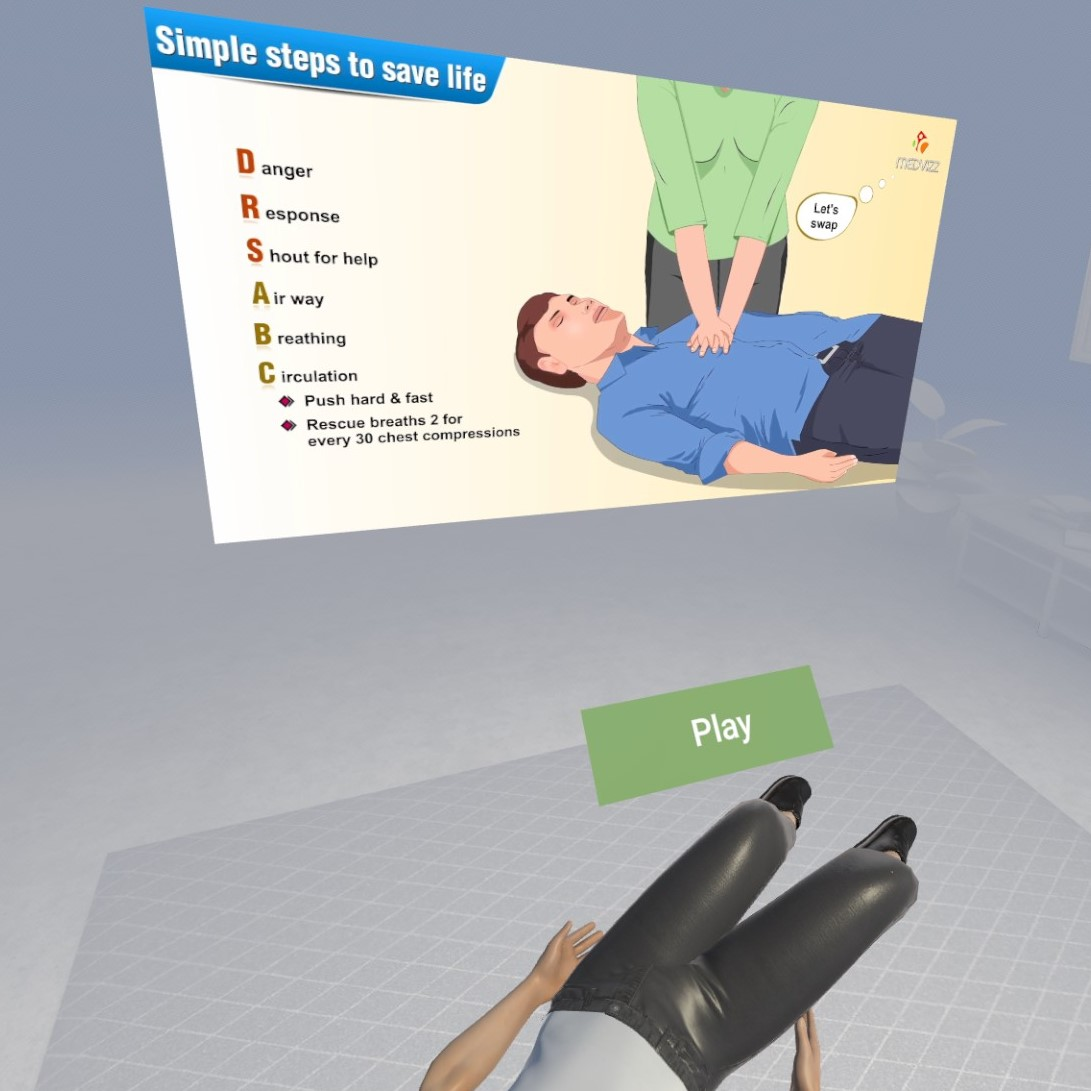
\includegraphics[width=\textwidth]{Photos/VR4.jpeg}
        \caption{Clear training videos}
        \label{fig:VR4}
    \end{subfigure}
    \caption{Virtual Reality scenario screenshots}
    \label{fig:overallVR}    
\end{figure}

\subsection{Design}
The independent variable in the study is training methodology, and the dependent variable in this experiment is CPR knowledge growth. The two factors, or controlled independent variables, are video-observation training and VR training. Given the nature of a between-group design, no counterbalancing was necessary. It is important to note the confounding variables: previous CPR knowledge, participant age, participant gender, and participant education. Altogether, 20 trials were administered for analysis. Once all the data was gathered, a python script ran several computations to compare the effects of each variable on the dependent variable.

\subsection{Testing Process}
Participants arrived at the testing facility, were informed that an experiment would be conducted, and were verbally asked if they consented to their participation. Before the experiment was conducted, each participant was informed about potential risks and the benefit of participation, and that this was completely voluntary, that they could leave at any time. The participants, one at a time, were positioned in front of the computer and instructed to follow the on-screen prompts. The facilitator would then assign a group number to the participant, according to a predetermined grid, and record it in the program to determine the path of the experiment. The participant would then answer a questionnaire that consisted of basic general questions about themselves, such as their age, education level, etc. After the questionnaire had concluded, the participant would have to answer 15 questions on the topic of CPR as a pre-assessment of knowledge. After the assessment had concluded, the participant would then deviate to the group assignment and either conduct training via VR or VOT, and both routes had identical training videos, varying only in medium. If the participant was selected to conduct training within the VR environment, they would have to read and accept the potential risks of the VR training. Once the training was complete, the participant would then have to answer 15 questions on the subject of CPR as a post-assessment of knowledge. After the post-assessment, a questionnaire was conducted to collect feedback on the experiment. The experiment would take about 15 minutes from start to finish. At the conclusion of the experiment, the participant was debriefed and dismissed.

\section{Results}
Five correlations were made from the data collected in this experiment. From this data, a combination of methods were utilized to extract a final outcome, which included running a Python script to turn the data into figures for the benefit of visualization and using online sources to analyze the data from a statistical standpoint, leading to key results.

\subsection{Data Summary}
A python script, found on the experiment's \href{https://github.com/csu-hci-projects/SP23-CPR-Resuscitation-Scenario-using-Virtual-Reality/blob/93a78caa6d9554e203a0d2402b1af35f86c4f6d5/DataAnalysis.py}{GitHub} repository, was created by the team to facilitate the creation of a few visual representations of the data in a style that is easy to read and is compliant with the Americans with Disabilities Act (ADA) \cite{kilin-2022}. The online statistical analysis tools that were deployed helped the team understand the inner workings of the data and helped analyze this data to come to a correlative conclusion. This online tool, found at the Statistics Kingdom website \cite{statistics-kingdom-2017}, processed and returned a representation of the data as well as easy-to-read figures. A decision was made to conduct a correlative analysis of five different relationships. These relations included: Training method vs. Test Scores, Training Method vs. CPR Comfort, CPR Comfort vs. Test Scores, Efficacy of Effect of Training Method on Test Scores, and Efficacy of Effect of Training Method on CPR Confidence. These correlative results are important, as they explain how the experiment is related to the final rejection or confirmation of the hypothesis. Overall, the data was not conclusive but did answer a few of the research questions previously mentioned, and the study was able to come to a correlative conclusion.

\subsubsection{Training Method vs. Test Scores}
\hfill\\
One noteworthy finding in this study revealed a slightly larger increase between Pre-Test results and Post-Test results in the VR trained group when compared to the video observation-trained group. The VR group test scores increased by 32.66 points, whereas the VOT group only increased by 26 points. Furthermore, the VR group actually started with a lower average on their Pre-Test scores (49.3 vs 52), but ended with a higher average than the VOT group on their Post-Test Scores (82 vs 78), as described in Figure \ref{fig:ScoresGraph}.

Another takeaway from the results shown in Figure \ref{fig:ScoresGraph} is that, while both groups had a comparable standard deviation for their Pre-Test scores, it was only the VR trained group that showed more precision in their Post-Test scores. The standard deviation for the VR group's Post-Test scores was only 6.69, while the VOT group's Post-Test scores standard deviation was 22.12. The standard deviation for the Pre-Test scores for the VR and VOT groups were 17.69 and 19.56, respectively.

\subsubsection{Training Method vs. CPR Comfort}
\hfill\\
When evaluating the different training method's potential correlations with overall CPR comfort, the average CPR comfort level for the VR group increases from 4 to 5.8, which is a 45\% increase in CPR confidence when trained using VR technology. Similarly, the VOT group increased their overall CPR comfort from 3.8 to 5.7, a 50\% increase.

The results in Figure \ref{fig:CPRComfortGraph} also show a comparable range when studying each group's standard deviation for both before and after their respective training. The standard deviation of each group's Pre-Test and Post-Test ranged between 2.4 and 3.25, a .85 difference.

\begin{figure}[h]
    \centering
    \begin{subfigure}[b]{0.4\textwidth}
        \centering
        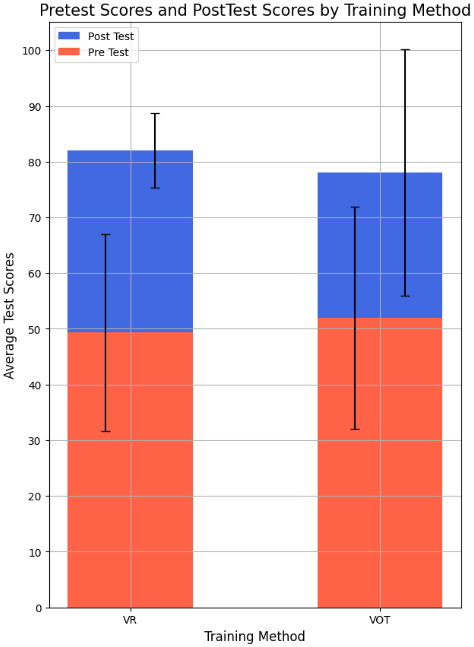
\includegraphics[width=\textwidth]{Photos/ScoresGraph.PNG}
        \caption{Pretest vs Posttest scores difference separated by training method.}
        \label{fig:ScoresGraph}
    \end{subfigure}
    \hfill
    \begin{subfigure}[b]{0.51\textwidth}
        \centering
        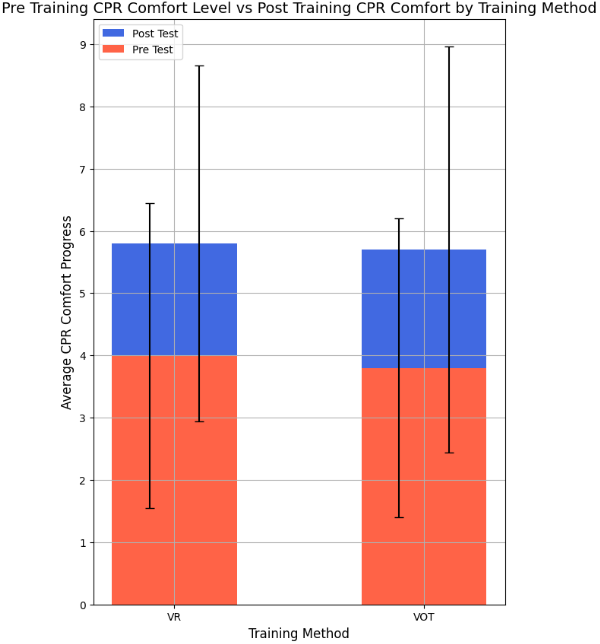
\includegraphics[width=\textwidth]{Photos/CPRComfortGraph.PNG}
        \caption{CPR Comfort Levels before and after training separated by training method.}
        \label{fig:CPRComfortGraph}
    \end{subfigure}
    \caption{Training Method impact on perceived CPR comfort and CPR test results}
\end{figure}

\subsubsection{CPR Comfort vs. Test Scores}
\hfill\\
Some interesting correlations reveal themselves when comparing each group's test progress to their respective CPR comfort progress. As seen in Figure \ref{fig:CPRGraph}, none of the participants scored lower on their test after training. Although, there were three individuals who reported less CPR comfort after training compared to how they felt about it prior to training.

Accounting for one outlier from each group, all other participants were able to provide a general trend indicated by the best fit line. In both cases of training method, the positive slope tells us that, in general, as participants became more knowledgeable in CPR, they also became more comfortable with performing CPR. Furthermore, the VOT group's best fit line shows a slightly higher ratio (.385 test points for every 1 CPR comfort point) than the VR group (.336 test points for every 1 CPR comfort point).

\begin{figure}[h]
    \centering
    \begin{subfigure}[b]{0.9\textwidth}
        \centering
        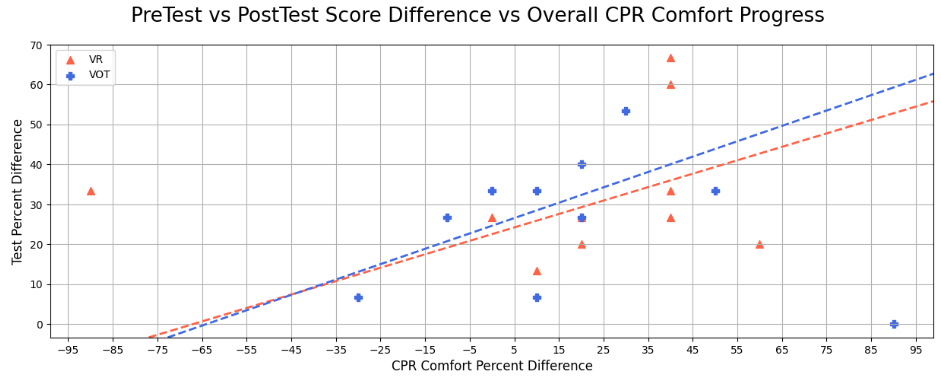
\includegraphics[width=\textwidth]{Photos/CPRGraph.PNG}
    \end{subfigure}
    \caption{CPR comfort level progress vs test results progress}
    \label{fig:CPRGraph}
\vspace{-2mm}
\end{figure}

\subsubsection{Efficacy of Effect of Training Method on Test Scores}
\hfill\\
To correlate the CPR test scores with the independent variable, the dependant variable of the CPR final test score was further evaluated by using the two-sample Mann-Whitney U test with normal distribution (two-tailed). It was concluded that they were not strong enough to conduct a t-test by calculating the normality of the two data residues, as illustrated in Table \ref{tab:MWTable1} as the dark red normality entry, which would have been a more powerful test to run on the data. Before running the statistical test, it was observed that the populations were not big enough to be statistically different since a minimum of 30 participants in each group is necessary. This indicated any data correlations would initially fail to reject the null hypothesis due to lack of data. 

\begin{figure}[!h]
    \centering
    \begin{subtable}[b]{.5\textwidth}
        \begin{tabular}{|p{.26\textwidth}||p{.3\textwidth}|p{.3\textwidth}|}
            \hline
            \multicolumn{3}{|c|}{VR Test Scores vs VOT Test Scores}\\
            \hline\hline
             & VR & VOT \\
            \hline
            Participants & 10 & 10\\            
            \hline
            Normality & \cellcolor{red!75}0.03909 & \cellcolor{green!75}0.4191\\
            \hline
            Rank & 108 & 102\\
            \hline
            U-Value & 47 & 53\\
            \hline\hline
            z-Value & 0.1913 &\\
            \hline
            P-Value & 0.8483 &\\
            \hline
        \end{tabular}
        \newline\newline
        \newline\newline
        \caption{Mann-Whitney U statistical analysis of training methods on assessment scores}
        \label{tab:MWTable1}
    \end{subtable}
    \hfill
    \begin{subfigure}[b]{.4\textwidth}
        \centering
        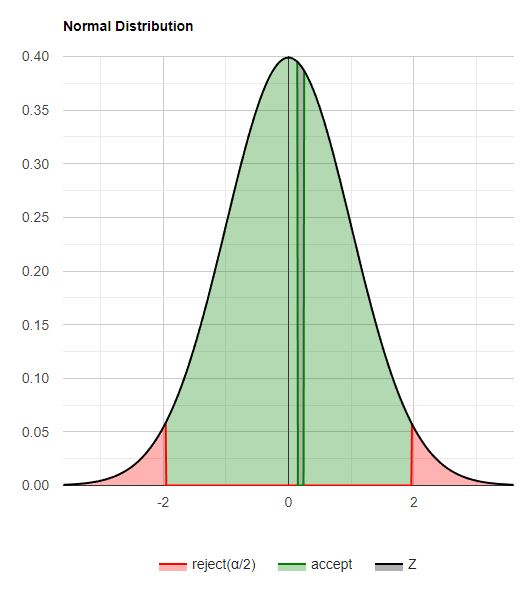
\includegraphics[width=\textwidth]{Photos/VR vs VOT group MWU test.jpg}
        \caption{Normal Distribution using Mann-Whitney U statistical analysis of training method on assessment scores}
        \label{fig:VR vs VOT group MWU test}
    \end{subfigure}
    \caption{Mann-Whitney U test results: Test Scores}
\end{figure}

To confirm this initial observation, the most appropriate parametric testing would be the Mann-Whitney U test with the help of the Wilcoxon rank-sum test for ranking purposes to define that the data is in a normal distribution range. According to Figure \ref{fig:VR vs VOT group MWU test}, the data from this experiment did fall within an acceptable, (light green) normal distribution. According to the data, the null hypothesis cannot be immediately rejected because the two ranks, 108 and 102, are not equal based on ranks alone. A z-Value of 0.1913 was determined and recorded in Table \ref{tab:MWTable1}. That z-value was then used to calculate the p-Value.

Finally, the p-Value of 0.8483, as seen in Table \ref{tab:MWTable1}, is significantly larger than the predefined significance level of 0.05, and thus fails to reject the null hypothesis. This means that the results were not significant enough to determine if the CPR test scores were affected by the experiment, confirming the initial observations about this dependant and independent variable correlation.

\subsubsection{Efficacy of Effect of Training Method on CPR Confidence}
\hfill\\
To correlate CPR confidence with the independent variable, the dependant variable of the CPR confidence score was observed by using the two-sample Mann-Whitney U test with normal distribution (two-tailed). This was calculated using the normality of the two data residues and concluded that they were not strong enough to conduct a t-test, illustrated in Table \ref{tab:MWTable2} as the dark red normality entry, which would have been a more powerful test to run on the data. Before running the statistical test, it was observed that the populations were not big enough to be statistically different, as a minimum of 30 participants in each group would be necessary. This meant that the results initially fail to reject the null hypothesis due to lack of data. 

\begin{figure}[!t]
    \centering
    \begin{subtable}[b]{.5\textwidth}
        \begin{tabular}{|p{.26\textwidth}||p{.3\textwidth}|p{.3\textwidth}|}
            \hline
            \multicolumn{3}{|c|}{Pre CPR Confidence vs Post CPR Confidence} \\
            \hline\hline
             & VR & VOT \\
            \hline
            Participants & 10 & 10\\
            \hline
            Normality & \cellcolor{red!75}0.006146 & \cellcolor{green!75}0.6475\\
            \hline
            Rank & 114.5 & 95.5\\
            \hline
            U-Value & 40.5 & 59.5\\
            \hline\hline
            z-Value & 0.6868 &\\
            \hline
            p-Value & 0.4922 &\\
            \hline  
        \end{tabular}
        \newline\newline
        \newline\newline
        \caption{Mann-Whitney U statistical analysis of training methods on CPR confidence scores}
        \label{tab:MWTable2}
    \end{subtable}
    \hfill
    \begin{subfigure}[b]{.4\textwidth}
        \centering
        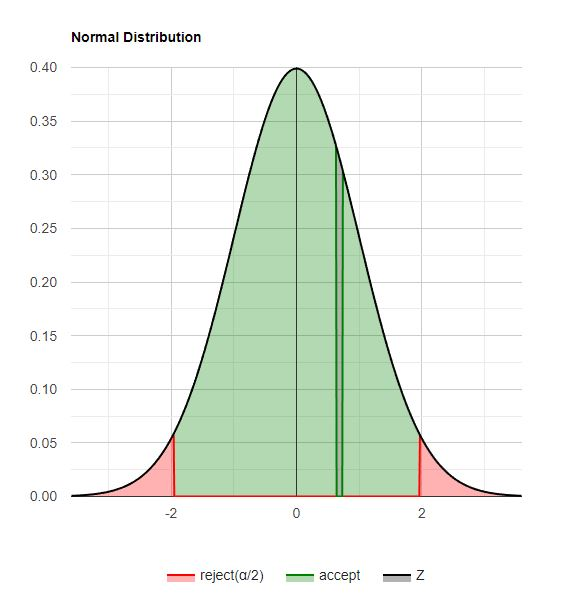
\includegraphics[width=\textwidth]{Photos/Pre CPR confidence VS Post confidence group MWU test.jpg}
        \caption{Normal Distribution using Mann-Whitney U statistical analysis of training method on CPR confidence scores}
        \label{fig:Pre CPR confidence VS Post confidence group MWU test}   
    \end{subfigure}
    \caption{Mann-Whitney U test results: CPR Confidence}
\end{figure}

To confirm this initial observation, The Mann-Whitney U test was used with the help of the Wilcoxon rank-sum test for ranking purposes to define that the data is in a normal distribution range. As observed in Figure \ref{fig:Pre CPR confidence VS Post confidence group MWU test}, the data from this experiment did fall within an acceptable, (light green) normal distribution. According to the data, the null hypothesis cannot be immediately rejected because the two ranks, 114.5 and 95.5, are not equal based on ranks alone. The z-Value was calculated to be 0.6868 and recorded in Table \ref{tab:MWTable2}. This z-Value was used to calculate the p-Value.

Finally, the p-Value was calculated to equal 0.4922, as seen in Table \ref{tab:MWTable2}, which is significantly larger than the predefined significance level of 0.05, and thus fails to reject the null hypothesis. This means that the results were not significant enough to determine if CPR confidence was affected by the experiment, confirming the initial observations about this dependant/independent variable correlation.

\subsection{Key Findings}
Upon closer review, the data revealed that VR training correlated with slightly improved CPR testing results and more consistent increases in CPR knowledge. On the other hand, neither training method showed a statistically significant difference in the growth of perceived CPR comfort. Additionally, as participants' CPR knowledge increased, so did their test performance. However, the VOT group showed slightly higher test-to-CPR-comfort progress. The effectiveness of the training methods on test scores and CPR confidence was not significant enough to conclusively determine whether the experiment influenced CPR confidence.

\section{Discussion}
In this study, the aim was to compare the effectiveness of VR Training and VOT for Cardiopulmonary Resuscitation (CPR) learners. The findings provide valuable insights into the potential benefits and limitations of using VR and VOT for CPR training, as well as areas for further research and improvement.

The findings revealed a correlation between VR training and somewhat improved CPR testing and more steady growth in CPR knowledge. Although perceived CPR comfort increased, neither training method demonstrated a statistically significant difference. The ability of participants to perform CPR effectively improved along with their CPR knowledge, while the VOT group demonstrated somewhat faster test-to-CPR-comfort development. Additionally, it should be noted that training variations would result in better performance on particular questions than the alternative. The results of this study are correlative rather than causative, indicating that a fundamental superiority of one training approach over the other could not be established.

The lack of statistical significance in some findings may be attributed to the small sample size and the fact that the data did not meet the normality assumptions for more powerful statistical tests. The lower overall experience score in the VR group may be attributed to participants adjusting to the VR environment for the first time, which could have distracted them from the CPR training. Additionally, the study's sample population may have limited the generalizability of the findings, as it was primarily composed of college-educated individuals between the ages of 20 and 40.

Despite these limitations, the results suggest that both VR and VOT can be effective methods for CPR training, with VR offering some advantages in terms of knowledge retention and test score improvement. However, further research with larger and more diverse sample sizes is needed to confirm these findings.

These findings contribute to the ongoing discussion about the effectiveness of various CPR training methods, including VR and VOT. While previous studies have reported mixed results, this study provides some support for the potential benefits of VR training in terms of improving CPR knowledge and test scores.

In summary, this study sheds light on the potential benefits and limitations of using VR and VOT for CPR training. While neither method demonstrated a clear advantage in terms of perceived comfort, VR training did show some promise for improving CPR knowledge and test scores. However, it is crucial to remember that the efficacy of training methods was not significant enough to determine their impact on CPR confidence. Future research should focus on larger and more diverse sample sizes, as well as addressing the limitations identified in this study, to better understand the effectiveness of each training method and their potential implications for CPR education.

\subsection{Limitations and Future Work}
The evaluations made in this study are mostly limited by time constraints. The researchers only had 5 months to implement the design, collect data, and summarize the results. As a consequence, time constraints and inexperience with programming in a VR environment limited the amount of interactions created for the dummy victim and equipment. More time should have been dedicated to the research behind the development of the VR portion of the experiment. 

In addition to allocating more time towards enhancing the VR aspect of the experiment, future research could also focus on improving the interaction points and feedback provided to participants during the simulation. For example, allowing participants to perform more realistic interactions with the victim inside VR, such as shaking the victim, pushing on the chest, or seeing the victim's mouth open and close in response to the participant's actions, could improve the immersion and effectiveness of the training. Also, by providing better feedback during the simulation, such as displaying panels or prompts that confirm the correct depth or compression rate of chest compressions, or the appropriate amount of breaths, could help participants retain techniques effectively. These improvements would require advanced programming and basic sensory feedback within the VR environment, but could ultimately lead to more realistic and effective training experiences.

The limited time also prevented the experiment from including all elements of current CPR training such as the Automated External Defibrillator (AED). The lack of AED may have made the more experienced participants question the integrity of the experiment. Future studies would benefit by integrating the AED into the simulation in order to have more realistic/up-to-date training. Additionally, due to the limited time available, the program could not be thoroughly alpha/beta tested, which may have caused poor feedback scores for the overall experience. 

The available supporting material for VOT was found to be conflicting or out of date, and while a video was selected that covered the basics and was taken from a reputable source, future studies should aim to identify a standardized training video. It should be acknowledged that there may be variations in CPR guidelines and techniques between different countries or regions, however, the fundamental principles and steps of CPR are consistent worldwide. Future research should prioritize the identification of reliable and standardized training material to ensure the accuracy of CPR.

The sample population was derived from the researchers' own network of social media contacts and as a result, the average education and age of the participants in this study mirrored that of the researchers. This may suggest that the results of this study may be more applicable to college-educated individuals between the ages of 20 and 40. The sample selection may also limit the generalizability of the findings to other populations with different age and educational backgrounds. In the future, it would be beneficial to have a bigger and more diverse sample size. Parametric tests were not applicable due to the non-normal distribution of the data. A larger sample size can improve statistical power, provide better data points for analysis, and reduce variance. Additionally, with a larger sample size, the data is more likely to conform to a normal distribution, making it easier to perform parametric tests such as t-tests. 

The study assessed participants' comfort level in performing CPR but did not collect data on prior CPR certification training. Since both CPR and VR are skills, it would have been beneficial to examine whether adapting to a VR environment for the first time could have distracted participants during the training. The lack of prior VR exposure might have contributed to the overall low experience score for the participants. In future studies, a section should be included that covers VR preliminary training, such as demonstrating how to click on buttons and navigating the environment.

Additionally, incorporating a control group that did not receive any form of training would have been valuable to the study. This would have allowed for a proper evaluation of the effectiveness of the different training methods.

\subsection{Acknowledgments}
This work is supported by Colorado State University, Fort Collins. We would like to acknowledge Francisco R. Ortega, Ph.D, Jacina Li, Richi Rodriquez, and our friends and family. We would also like to express our gratitude to the Computer Science department for their support in providing us with the necessary virtual reality equipment, including the Meta Quest 2 headset, to conduct our research.

\bibliographystyle{./Citations/ACM-Reference-Format}
\bibliography{./Citations/CPRProjectCitations}

\end{document}
\endinput
%%
%% End of file `Cardiopulmonary-Resuscitation-Scenario-using-Virtual-Reality.tex'.